\documentclass[class=scrbook, crop=false]{standalone}
\usepackage[subpreambles=true]{standalone}
\ifstandalone
    % ---------------------------------------------------------------------
% File Import Support
% ---------------------------------------------------------------------
\usepackage{import} % Enables relative path imports for modular document structure.

% ---------------------------------------------------------------------
% Language and Character Encoding
% ---------------------------------------------------------------------
\usepackage[ngerman, english]{babel} % Set document languages: German + English.

% ---------------------------------------------------------------------
% Font Configuration — LuaLaTeX Only
% ---------------------------------------------------------------------
% LuaLaTeX handles UTF-8 input natively — inputenc and fontenc are obsolete here.

\usepackage{lmodern}   % Default serif/monospace fallback fonts.
\usepackage{fontspec}  % Primary font package for LuaLaTeX.
\setsansfont{Liberation Serif}    % Set sans-serif font to Arial (main font for this document).

% Notes:
% - lmodern fills in main and monospace fonts if not explicitly set with fontspec.
% - Comment lmodern if full fontspec control is preferred.

% ---------------------------------------------------------------------
% Page Layout and Formatting
% ---------------------------------------------------------------------
\usepackage[automark,headsepline]{scrlayer-scrpage} % Header/footer management.

\newcommand{\theBCOR}{15mm} % Binding correction for double-sided print layouts.

\usepackage[
    bindingoffset=\theBCOR,
    % showframe, % Show boxes which indicate margins and paddings
    bottom = 3.5cm,
    left = 2.5cm,
    right = 2.5cm
]{geometry} % Custom page dimensions.

\usepackage{float}          % Prevent page breaks inside figures/tables.
\usepackage{pdflscape}      % Landscape page support.
\usepackage{threeparttable} % Table notes support.
\usepackage{booktabs}       % Improved table rules and spacing.

% ---------------------------------------------------------------------
% Content Presentation
% ---------------------------------------------------------------------
\usepackage{tikz}          % Graphics and diagrams.
\usepackage{graphicx}      % Image inclusion.

\addtokomafont{disposition}{\rmfamily} % Roman font for all section headings.

\usepackage[onehalfspacing]{setspace}  % Line spacing: 1.5x for readability.

\usepackage[stretch=10]{microtype}     % Typographic optimizations.
% Disable expansion if font glitches occur:
% \usepackage[stretch=10, expansion=false]{microtype}

\usepackage{textcomp}      % Access to symbols like \textmu (µ).

\usepackage[
    range-units=single,
    range-phrase=-,
    separate-uncertainty=true,
    multi-part-units=repeat
]{siunitx} % Scientific units, uncertainty handling.
% https://tex.stackexchange.com/questions/124488/multi-part-numbers-and-units-in-siunitx

\usepackage{listings}      % Source code formatting.
\usepackage{enumitem}      % Fine-tune list spacing and indentation.
\setlist{nosep}

\usepackage{todonotes}     % Inline ToDo notes.
\setuptodonotes{inline, inlinepar}
\reversemarginpar          % Place ToDo notes in the left margin.
% Adjust margin width if notes overflow:
% \setlength{\marginparwidth}{2cm}

\usepackage{xcolor}        % Color customization support.
\usepackage{amsmath}       % Math typesetting.

% ---------------------------------------------------------------------
% Utility Packages
% ---------------------------------------------------------------------
\usepackage{blindtext}     % Filler text for layout development.
\usepackage[hidelinks]{hyperref} % Hide link borders in PDF output.

% ---------------------------------------------------------------------
% Glossary and Index
% ---------------------------------------------------------------------
% IMPORTANT: Version pin required for compatibility.
\usepackage[acronym, nogroupskip]{glossaries}[=v4.49]
\usepackage{xltabular}     % Required table layout extension for glossaries.

% ---------------------------------------------------------------------
% Bibliography Configuration
% ---------------------------------------------------------------------
\usepackage{csquotes}      % Quotation style integration.
\usepackage[
    style=ieee,
    citestyle=numeric-comp,
    backend=biber
]{biblatex}

% ---------------------------------------------------------------------
% Chair specific Packages — Automatically enabled via \selectchair
% ---------------------------------------------------------------------
\ifchair{SYSCOP}
    \usepackage{optidef} % Package to write optimization problems
    \usepackage{amsfonts} % extended set of fonts for use in mathematics
\fi

% ---------------------------------------------------------------------
% Paths and Included Files
% ---------------------------------------------------------------------
% Fix paths for standalone compiling
\ifstandalone
    \def \home {..}
\else
    \def \home {.}
\fi

\input{\home/settings+/style/page}     % Page style configuration.
\graphicspath{{\home/images/}}         % Default image path.

\input{\home/settings+/style/code.tex} % Code listings style.
\lstset{inputpath={\home/code/}}       % Default path for listings files.

\input{\home/settings+/style/symbols}       % Set path to symbols list style file
\input{\home/settings+/style/acronyms}      % Set path to acronym list style file
\input{\home/references/glossary_acronyms}  % Load glossary, symbol and acronyms list

\addbibresource{\home/references/references.bib}
\input{\home/settings+/variables}

\usepackage[listings=false]{scrhack} % Compatibility fix for older packages.

% ---------------------------------------------------------------------
% Optional Packages — Comment/Uncomment As Needed
% ---------------------------------------------------------------------
% \usepackage{amsfonts}      % Additional mathematical fonts
% \usepackage{caption}       % Customize caption appearance for figures and tables
% \usepackage{subcaption}    % Create subfigures/subtables with individual subcaptions
% \usepackage{calc}          % Arithmetic with LaTeX lengths.
% \usepackage{imakeidx}      % Index creation.
% \usepackage{paralist}      % Compact lists.
% \usepackage{epigraph}      % Quotation formatting.
\usepackage{algorithm}     % Algorithms (floating).
\usepackage{algpseudocode} % Pseudocode formatting.
% \usepackage{algorithmic}   % Legacy pseudocode.
% \usepackage{xspace}        % Smart space insertion.
% \usepackage{tabularx}      % Flexible table widths.
% \usepackage{longtable}     % Multipage tables.
% \usepackage{verbatim}      % Multiline comments.
% \usepackage{datapie}       % Pie charts.
% \usepackage{afterpage}     % Command placement after page breaks.
% \usepackage{wrapfig}       % Text wrapping around figures.
\usepackage{amsthm}
\usepackage{graphicx}
\usepackage{subcaption}
\usepackage{nicematrix}

\theoremstyle{plain}
\newtheorem{remark}{Remark}
\newtheorem{assumption}{Assumption}
\newtheorem{theorem}{Theorem}
\newtheorem{lemma}[theorem]{Lemma}
\newtheorem{proposition}[theorem]{Proposition}
\fi

% ----------------------------------------------------------------------------
%                               Results
% ----------------------------------------------------------------------------
\begin{document}

\chapter{Numerical experiments} % Overview text
\label{Chapter::Experiments}
In this chapter, we evaluate the proposed regularization methods numerically and discuss the results.
We begin in Section~\ref{sec:metrics} with the two metrics used throughout the comparison, 
the iteration profile and the flop unit estimation, which measure convergence behavior and factorization cost respectively.
Section~\ref{sec:prototype} then describes the prototype solver on which all experiments are run 
and establishes that it reproduces the iteration behavior of HPIPM on convex QPs, 
so that any difference observed later can be attributed to the regularization rather than to the solver itself.
Section~\ref{sec:setup} fixes the experiment setup, 
naming and classifying the regularization methods under comparison and stating the parameters shared by all of them.
Section~\ref{sec:comparison} presents the numerical comparison, 
first among the Riccati-based methods themselves and then against full Hessian regularization and inertia correction.
Section~\ref{sec:discussion} concludes the chapter by discussing what distinguishes the hard instances from the easy ones 
and why the full Hessian methods perform poorly.

\section{Experiment metrics}
\label{sec:metrics}
In this section, we will introduce the metrics used to evaluate the performance of different regularization strategies in our experiments.
Since we care about both the convergence behavior and the factorization cost caused by different regularization methods, 
we will use two complementary metrics: iteration profile and flop unit estimation.
The former one, iteration profile, is used to evaluate how many iterations each method takes to converge on a set of test instances, 
while the latter one, flop unit estimation, is approximated by the number of modified Cholesky factorization of the reduced Hessian, which is used to evaluate the factorization cost of each method.

\subsection{Iteration profile}
Let $\mathcal{P}$ denote the set of test instances and $\mathcal{M}$ the set
of candidate regularization strategies. For a method $m \in \mathcal{M}$ and
an instance $\mathrm{p} \in \mathcal{P}$, let $i_{m,\mathrm{p}}$ be the number of
iterations $m$ needs to satisfy the convergence criterion on $\mathrm{p}$.
If the run reaches the iteration cap $i_\mathrm{max}$, the instance is counted as unsolved and $i_{m,\mathrm{p}}=\infty$.
The \emph{iteration profile} of method $m$ is
\begin{equation}
\Pi_m(\ell) \;=\; \bigl|\{\, \mathrm{p} \in \mathcal{P} : i_{m,\mathrm{p}} \le \ell \,\}\bigr|,
\qquad \ell = 1,\dots,i_\mathrm{max},
\end{equation}
i.e.\ the number of instances that $m$ solves within $\ell$ iterations.
A curve that rises steeply at small $\ell$ indicates an \emph{efficient} method,
and its final value $\Pi_m(i_\mathrm{max})$, the number of solved instances,
measures its \emph{robustness}.

\subsection{Flop unit estimation}
Iteration counts alone do not reflect the work performed per iteration,
which differs substantially across regularization strategies: an
eigenvalue-based correction and a modified-Cholesky correction may reach
convergence in a comparable number of iterations while incurring very
different arithmetic cost. To compare methods on a common scale, we express
the cost of all matrix factorizations and decompositions in a single flop unit.

We take one modified Cholesky factorization of the block reduced Hessian as
the unit. For a control dimension $n_u$, factorizing an $n_u \times n_u$
matrix costs approximately $\tfrac{1}{3} n_u^3$ flops, hence
\begin{equation}
\mathrm{unit} \;\approx\; \tfrac{1}{3}\, n_u^3 .
\end{equation}
The modified factorization differs from the plain one only by lower-order
diagonal updates, so to leading order it also costs one unit.

The remaining primitives are expressed relative to this unit. A symmetric
eigenvalue decomposition of the same block costs about $9 n_u^3$ flops
\cite{verschuerenTimeoptimalRaceCar2016b}, i.e.
\begin{equation}
\frac{9 n_u^3}{\tfrac{1}{3} n_u^3} \;=\; 27 \ \text{units}.
\end{equation}
Regularizing the cost-to-go matrix $P_{k+1} \in \mathbb{R}^{n_x \times n_x}$
or a full Hessian block $\tilde{H}_k \in \mathbb{R}^{(n_x+n_u) \times (n_x+n_u)}$
applies the same primitives to a larger block. With the ratios
\begin{equation}
\omega_P \;=\; \left(\frac{n_x}{n_u}\right)^{3}, \qquad
\omega_H \;=\; \left(\frac{n_x+n_u}{n_u}\right)^{3},
\end{equation}
a modified Cholesky factorization of $P_{k+1}$ costs $\omega_P$ units and an eigenvalue decomposition $27\omega_P$ units,
and likewise $\omega_H$ and $27\omega_H$ units for $\tilde{H}_k$.
Since the full Hessian regularization modifies all $N$ blocks $\tilde{H}_k$ at once,
each regularization costs $N\omega_H$ or $27N\omega_H$ units.
The cost of a solve is the total number of units accumulated over all its iterations.

\section{Prototype solver implementation}
\label{sec:prototype}
To unify the comparison, we implemented a prototype solver capable of accommodating all regularization methods under consideration. 
The Riccati-based primal-dual interior-point solver is implemented in Python, using HPIPM, 
the state-of-the-art Riccati-based IPM solver for OCP QPs, as a reference. 
The prototype was designed to reproduce its iteration behavior on convex QPs, where the two solvers should therefore agree.
It is available at \url{https://github.com/Pandatheon/Primal-dual_IPM.git}.

One implementation detail deserves mention, as it departs from the plain FTB rule stated in Section~\ref{sec:size_control}. 
Rather than retracting the maximal step by a fixed fraction $\eta$, 
the primal and dual step sizes $\alpha_{\mathrm{prim}}$ and $\alpha_{\mathrm{dual}}$ are each obtained 
from their respective maximal step through the heuristic
\begin{equation}
  \alpha =
  \begin{cases}
    \alpha_{\mathrm{max}}\big[(1-\alpha_{\mathrm{max}})\,\kappa_\eta + \alpha_{\mathrm{max}}\hat{\eta}\big], & \alpha_{\mathrm{max}} < 1,\\
    \alpha_{\mathrm{max}}, & \alpha_{\mathrm{max}} = 1,
  \end{cases}
\end{equation}

where $\alpha_{\mathrm{max}}\in(0,1]$ denotes the maximal step length for ensuring the positivity of the slack and dual variables, 
$\kappa_\eta = 0.99$ and $\hat{\eta} = 1-10^{-7}$.
The bracketed factor interpolates linearly between the conservative constant $\kappa_\eta$ and the near-unit value $\hat{\eta}$, 
with $\alpha_{\mathrm{max}}$ itself as the interpolation weight.
The separate case $\alpha_{\mathrm{max}} = 1$ is needed, 
otherwise the first branch would scale an unblocked full step by $\hat{\eta}$ and prevent it from ever being taken exactly, 
thus affecting the local qudratic convergence rate of IPM.

For the comparison to be meaningful, 
We align the prototype solver with HPIPM in terms of the algorithmic choices.
We therefore define a set of HPIPM settings, referred to in the following as the \texttt{CUSTOMIZED} mode, 
the values are listed in Table~\ref{tab:customized_settings}.


\begin{table}[H]
\caption{Detailed settings for the defined \texttt{CUSTOMIZED} mode.}
\label{tab:customized_settings}
\centering
\begin{tabular}{ll|ll}
\toprule
\textbf{Parameter} & \textbf{Value} & \textbf{Parameter} & \textbf{Value} \\ 
\midrule
\texttt{mu0} & \texttt{1e1} & \texttt{lam\_min} & \texttt{1e-12} \\
\texttt{alpha\_min} & \texttt{1e-12} & \texttt{t\_min} & \texttt{1e-12} \\
\texttt{res\_g\_max} & \texttt{1e-6} & \texttt{tau\_min} & \texttt{1e-12} \\
\texttt{res\_b\_max} & \texttt{1e-8} & \texttt{lam0\_min} & \texttt{1e-12} \\
\texttt{res\_d\_max} & \texttt{1e-8} & \texttt{t0\_min} & \texttt{1e-12} \\
\texttt{res\_m\_max} & \texttt{1e-6} & \texttt{warm\_start} & \texttt{0} \\
\texttt{dual\_gap\_max} & \texttt{1e15} & \texttt{abs\_form} & \texttt{0} \\
\texttt{iter\_max} & \texttt{30} & \texttt{comp\_dual\_sol\_eq} & \texttt{1} \\
\texttt{stat\_max} & \texttt{30} & \texttt{comp\_res\_exit} & \texttt{1} \\
\texttt{pred\_corr} & \texttt{1} & \texttt{comp\_res\_pred} & \texttt{1} \\
\texttt{cond\_pred\_corr} & \texttt{1} & \texttt{split\_step} & \texttt{1} \\
\texttt{itref\_pred\_max} & \texttt{0} & \texttt{m\_safe} & \texttt{0.5} \\
\texttt{itref\_corr\_max} & \texttt{0} & \texttt{var\_init\_scheme} & \texttt{0} \\
\texttt{reg\_prim} & \texttt{0.0} & \texttt{t\_lam\_min} & \texttt{2} \\
\texttt{square\_root\_alg} & \texttt{0} & \texttt{t0\_init} & \texttt{2} \\
\texttt{lq\_fact} & \texttt{0} & \texttt{update\_fact\_exit} & \texttt{1} \\ 
\bottomrule
\end{tabular}
\end{table}

As one can notice, the \texttt{CUSTOMIZED} mode largely coincides with the \texttt{SPEED} mode of the original HPIPM, differing in two respects. 
First, the square-root algorithm is disabled (\texttt{square\_root\_alg}$=0$), 
so that the Riccati recursion is carried out directly rather than on Cholesky factors.
Second, the primal and dual step sizes are computed separately (\texttt{split\_step}$=1$) instead of sharing a single step length.
In both modes no iterative refinement is applied to the predictor or corrector steps (\texttt{itref\_pred\_max}$=$\texttt{itref\_corr\_max}$=0$) 
and no default primal regularization is added (\texttt{reg\_prim}$=0$), 
while Mehrotra's predictor--corrector is retained and applied conditionally (\texttt{pred\_corr}$=$\texttt{cond\_pred\_corr}$=1$).

To verify that the two implementations do agree, we collected $40$ convex QP subproblems, 
five from each of the $8$ OCPs in the benchmark, 
and compared the iteration behavior of the prototype solver against that of \texttt{CUSTOMIZED}-mode HPIPM. 
The resulting iteration profiles are shown in Figure~\ref{fig:convex_iteration_profile}. 

Both solvers solve all $40$ instances in the exact same number of iterations for each instance, 
resulting in performance profiles that coincide across the whole budget range, from $4$ up to $22$ iterations. 
On convex QPs the prototype solver therefore reproduces the iteration behavior of HPIPM, 
which verifies the prototype as a reliable baseline 
and allows us attribute the differences observed in the experiments to the regularization rather than to the solver.

\begin{figure}[H]
    \centering
    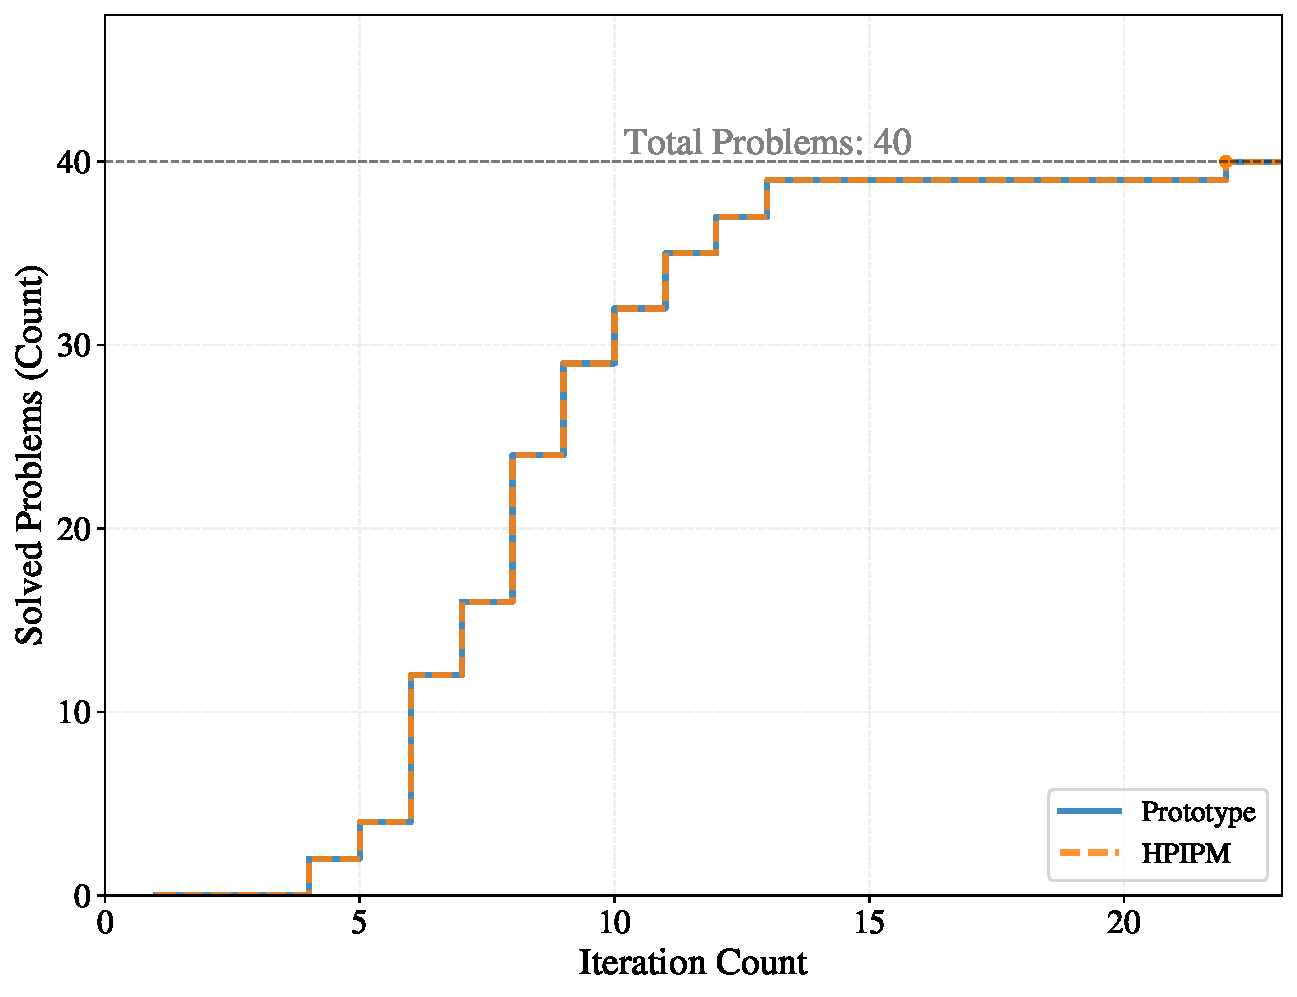
\includegraphics[width=0.75\textwidth]{images/experiment/convex_qp/iteration_qp_results_pos.pdf}
    \caption{Iteration profiles on 40 convex QPs. The prototype solver is compared with HPIPM, showing identical iteration behavior.}
    \label{fig:convex_iteration_profile}
\end{figure}


\section{Experiment setup}
\label{sec:setup}
In this section, 
the settings preparation for the experiment are introduced.
First, based on the previously discussed methods, 
we will name and classify the regularization methods considered in the experiment, 
then we will introduce the general setup of the experiments, including the convergence criterion and step-size control strategy.

\subsection{Experimented regularizations}
\label{subsec:experimented_regularizations}
Before turning to the results, we fix the set of regularization methods entering the comparison, 
together with the naming convention used throughout this chapter.

Following the classification in Section~\ref{sec:hessian_reg}, 
the methods are grouped by their \emph{target}, 
that is, by the matrix whose indefiniteness the correction is derived from and to which the correction is directly applied, 
rather than by how the correction itself is computed. 
This yields three families: full Hessian regularization, Riccati-based regularization, and inertia correction.
The numerical strategies of Section~\ref{subsec:reg_strategies}, 
namely spectral projection (\textsf{PROJECT}), eigenvalue mirroring (\textsf{MIRROR}) 
and the Gill--Murray--Wright modified Cholesky factorization (\textsf{GMW}), 
are largely independent of the matrix they act on and can therefore be paired with each target.

Every method is accordingly named in the form \textsf{TARGET\_STRATEGY}, 
so that both factors can be read off directly from the label, 
and the comparison can be carried out either across targets at a fixed strategy or across strategies at a fixed target.

\paragraph{Full Hessian Regularization}
The first family follows Section~\ref{subsec:full_hessian} and enforces positive definiteness of the full Hessian $\tilde{H}$ in the KKT system.
The regularization is also triggered by the failure of the Choleksy factorization in Riccati recursion,
the regularized full Hessian is obtained by stage-wisely regularizing each block $\tilde{H}_k$ and 
the Riccati recursion is re-attempted with it. The three variants differ only in how the block adjustment $E_k$ is formed:

\begin{itemize}
    \item \textsf{H\_PROJECT}: the negative and near-zero eigenvalues of each $\tilde{H}_k$ are clipped to $\epsilon$, 
    which gives the smallest perturbation in Frobenius norm that restores positive definiteness.
    \item \textsf{H\_MIRROR}: the eigenvalues of each $\tilde{H}_k$ are replaced by their absolute values (floored at $\epsilon$), 
    which preserves the magnitude of the curvature along every eigendirection at the price of a larger modification.
    \item \textsf{H\_GMW}: the diagonal pivots of each $\tilde{H}_k$ are bounded from below during the $\mathrm{LD}\mathrm{L}^\top$ factorization, 
    which avoids an eigendecomposition altogether and keeps the entries of the triangular factor bounded, 
    but yields a non-minimal, ordering-dependent perturbation.
\end{itemize}

\paragraph{Riccati-based Regularization}
The second family is the one proposed in Section~\ref{sec:riccati_primal_reg} and acts on the reduced Hessian $\tilde{M}$.
The algorithms are given in Algorithms~\ref{alg:modified_riccati_recursion} and \ref{alg:improved_modified_riccati_recursion},
where the regularization is applied stage-wise to the block reduced Hessian $\tilde{M}_k$ during the backward pass, 
when the failure of the Cholesky factorization of $\tilde{M}_k$ occurs.

The two algorithms differ in which matrices of the backward pass the adjustment is derived from and applied to, 
giving two targets within this family:
\begin{itemize}
  \item \textsf{M}: only the block reduced Hessian $\tilde{M}_k$ is corrected, as in Algorithm~\ref{alg:modified_riccati_recursion}. 
  The correction is purely local and serves as a minimal safeguard for the factorization.
  \item \textsf{PM}: the cost-to-go matrix $P_{k+1}$ entering the stage is corrected as well, 
  as in Algorithm~\ref{alg:improved_modified_riccati_recursion} introduced in this work, 
  so that the propagation of negative curvature analysed in Section~\ref{sec:fail_minimal_perturbation} 
  is accounted for consistently in $\tilde{M}_k$, $\Gamma_k$ and $P_k$.
\end{itemize}

Pairing each target with the three strategies gives the six methods compared in this chapter. 
Each method accordingly answers a specific question in the comparison based on the insights mentioned in Section~\ref{sec:fail_minimal_perturbation}:

\begin{itemize}
  \item \textsf{M\_PROJECT}: the reference point of the family. 
  A minimum-norm correction applied locally is the naive and cheapest way to enforce positive definiteness,
  and is the configuration that the analysis of Section~\ref{sec:fail_minimal_perturbation} predicts to be the most exposed to condition-number growth.
  \item \textsf{M\_MIRROR}: whether abandoning the minimum-perturbation rule is by itself sufficient, with the propagation left untreated.
  \item \textsf{M\_GMW}: the same question as \textsf{M\_MIRROR}, but with the correction on the inertia of the factorization rather than on the spectrum, 
  which indicates whether the cheaper Type-II correction can stand in for mirroring.
  \item \textsf{PM\_PROJECT}: conversely, whether regularizing the cost-to-go matrix helps even when the minimum-perturbation rule is retained, 
  so that this case can be discussed rather than merely argued for.
  \item \textsf{PM\_MIRROR}: both insights combined, and thus the method the analysis of Section~\ref{sec:fail_minimal_perturbation} recommends.
  \item \textsf{PM\_GMW}: combines both insights with a cheaper factorization-based correction 
  to explore the trade-off between robustness and decomposition cost compared to \textsf{PM\_MIRROR}.
\end{itemize}

\paragraph{Inertia Correction}
The third family is the Levenberg--Marquardt style inertia correction used in IPOPT~\cite{wachter2006implementation}, 
which we denote by \textsf{INERTIA\_LM} and take as the practical reference point for the comparison.

In this strategy, a scalar multiple of the identity $\delta_w I$ is added stage-wise to the full Hessian, 
i.e.\ each full Hessian block $\tilde{H}_k$ is replaced by $\tilde{H}_k + \delta_w I$, 
and the Riccati recursion is repeated with increasing $\delta_w$ until it succeeds.
Only the primal regularization from IPOPT is retained, 
as dual regularization is not the primary focus of this work.

Notably, the method sits between the two preceding families, as it has no distinct target matrix in the above sense. 
Being a uniform multiple of the identity, the shift is not tied to any particular direction, 
so the perturbation remains a uniform shift along every direction for both the full and the reduced Hessian. 
Accordingly, as $\delta_w I$ is applied uniformly to $Q_k$ and $R_k$ in full Hessian blocks $\tilde{H}_k$, 
it enters the Riccati recursion as the same additive term on the reduced Hessian blocks $\tilde{M}_k$ and $P_k$.

The trial sequence follows IPOPT as well: 
the unmodified matrix is attempted first ($\delta_{\mathrm{LM}} = 0$), 
the first correction of a solve starts from $\delta_w^0$ and is then scaled by the accelerated factor $\bar{\kappa}_w^+$, 
subsequent corrections are scaled by $\kappa_w^+$ until the Riccati recursion succeeds or the threshold $\delta_w^{\max}$ is exceeded, 
and a successful value is stored and reduced by $\kappa_w^-$ as the starting point of the next iteration. 
The parameters are set to the IPOPT defaults and are listed in Table~\ref{tab:inertia_correction}.

\begin{table}[H]
  \centering
  \caption{Inertia Correction (IC) Parameters}
  \label{tab:inertia_correction}
  \vspace{0.5em}
  \begin{tabular}{ccp{10cm}}
    \toprule
    \textbf{Symbol} & \textbf{Value} & \textbf{Description} \\
    \midrule
    $\delta_w^0$        & $10^{-4}$  & Initial Hessian perturbation parameter \\
    $\delta_w^{\min}$   & $10^{-16}$ & Minimum allowable regularization parameter \\
    $\delta_w^{\max}$   & $10^{16}$  & Maximum allowable regularization threshold \\
    $\kappa_w^-$        & $1/3$      & Factor to decrease perturbation upon success \\
    $\kappa_w^+$        & $8$        & Factor to increase perturbation after inertia failure \\
    $\bar{\kappa}_w^+$  & $10^2$     & Accelerated scaling factor for severe indefiniteness \\
    $\delta_{\text{LM}}$& $0.0$      & Initial LM shift (IC-1: attempt unmodified matrix first) \\
    \bottomrule
  \end{tabular}
\end{table}

Taken together, the three families span ten methods, 
which share the same solver, the same benchmark and the same parameters introduced in the next subsection, 

\subsection{General setup}
All ten methods are run under the same conditions. 
The barrier parameter is updated by Mehrotra probing 
and the step size is controlled by the FTB rule followed by the two-phase line search, 
while the remaining settings are collected in Table~\ref{tab:general_settings}.

A run terminates either when all four residuals fall below their tolerances 
or when the iteration budget $i_\mathrm{max}$ is exhausted, in which case the instance counts as unsolved.

\begin{table}[H]
\centering
\caption{Settings shared by all experiments.}
\label{tab:general_settings}
\vspace{0.5em}
\begin{tabular}{ccp{7.5cm}}
    \toprule
    \textbf{Symbol} & \textbf{Value} & \textbf{Role} \\
    \midrule
    $r_\mathrm{stat}$  & $10^{-6}$ & Tolerance on the stationary residual \\
    $r_\mathrm{eq}$    & $10^{-8}$ & Tolerance on the equality residual \\
    $r_\mathrm{ineq}$  & $10^{-8}$ & Tolerance on the inequality residual \\
    $r_\mathrm{comp}$  & $10^{-6}$ & Tolerance on the complementarity residual \\
    \addlinespace
    $i_\mathrm{max}$   & $120$     & Iteration budget, beyond which the instance counts as unsolved \\
    $n_\mathcal{P}$    & $175$     & Nonconvex QP instances in the test set \\
    \addlinespace
    $\epsilon$         & $10^{-4}$ & Floor on the corrected eigenvalues and pivots, shared by all strategies \\
    \addlinespace
    $\beta$           & $0.5$      & Backtracking factor, $\alpha_\mathrm{prim} \leftarrow \beta\alpha_\mathrm{prim}$ \\
    $n_\mathrm{max}$        & $10$        & Maximum backtracking iterations \\
    $\kappa_s$      & $10^{-1}$  & Switching constant, $\alpha_\mathrm{prim}(-\rho) > \kappa_s\,\theta^2$ \\
    $\gamma$        & $10^{-4}$  & Armijo constant for the f-phase, $f^+ \le f + \gamma\,\alpha_\mathrm{prim}\rho$ \\
    \bottomrule
\end{tabular}
\end{table}

\section{Numerical comparison}
\label{sec:comparison}
In this section, we report the numerical results of the ten regularization methods on the nonconvex QPs of the benchmark.
The comparison proceeds in three stages, each narrowing the field. 
We first compare the six Riccati-based methods against one another, 
in order to identify the strongest representatives of the family. 
These are then set against the full Hessian regularizations, 
and finally against inertia correction, which serves as the practical reference point.

\subsection{Comparison among Riccati-based regularizations}
We first compare the proposed Riccati-based regularization methods, 
which are the main focus of this work.
As a baseline we also include the unregularized recursion (\textsf{NO\_REGULARIZE}). 

The iteration profile in Figure~\ref{fig:iter-profile-riccati} reports, 
for each method, the number of instances solved within a given iteration budget, where two trends stand out. 
First, each \textsf{PM} dominates its counterpart \textsf{M} once the budget exceeds about $30$ iterations, 
second, among the regularization strategies, \textsf{MIRROR} and \textsf{GMW} are clearly more effective than \textsf{PROJECT}.
These trends validate the insights mentioned in Section \ref{sec:fail_minimal_perturbation}.
Among all the methods, \textsf{PM\_MIRROR} tops the profile, solving $171$ of the $175$ instances, 
with \textsf{PM\_GMW} close behind at $167$.

Besides, it is interesting to note that 
the unregularized recursion can also solve a non-negligible fraction of the test set ($31$ of the $175$ instances),
which can be explained by the curvature contribution of the constraint that help to make the reduced Hessian positive definite in some instances.

\begin{figure}[H]
    \centering
    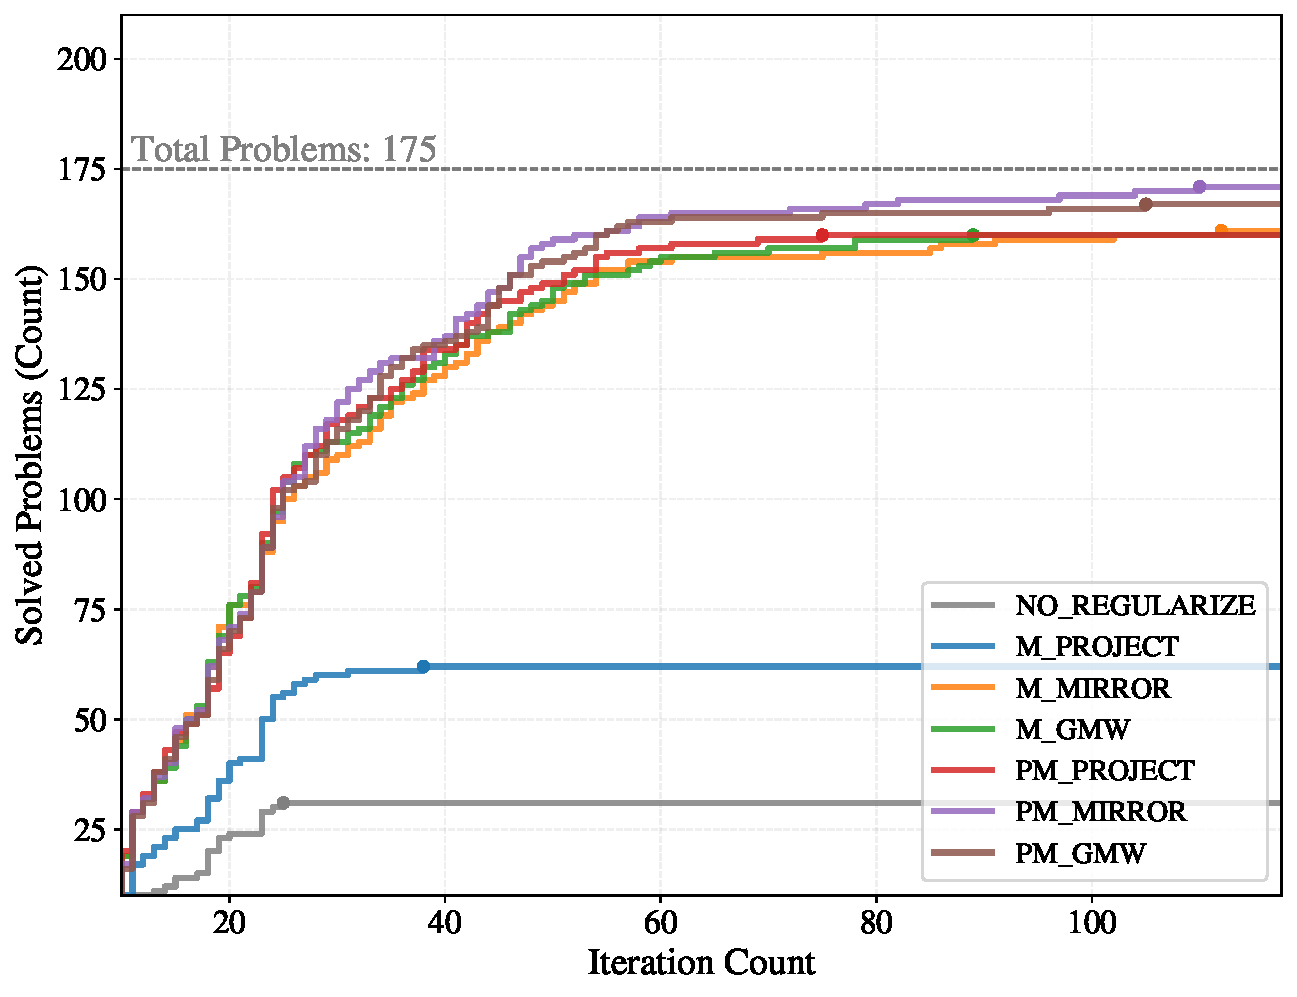
\includegraphics[width=0.8\textwidth]{images/experiment/Riccati-based_results/iteration_qp_results_riccati.pdf}
    \caption{Iteration profile of the six Riccati-based methods over the $175$-instance test set:
    number of instances solved within a given iteration budget.}
    \label{fig:iter-profile-riccati}
\end{figure}

Figure~\ref{fig:flop-profile-riccati} complements this picture by showing the distribution of the worst-case decomposition cost in flop estimation, 
annotated with the maximum observed cost and the number of failures for each method.
Since only the successful instances and maximal iteration instances are counted,
the \textsf{M\_PROJECT} will be excluded from the anaylsis, due to the frequent failing on $113$ of the $175$ instances.

In general, the \textsf{PM} incur a higher and more dispersed cost, reflecting the extra factorization work introduced by the cost-to-go term, 
yet they are generally more robust and thus the focus of the comparison. 
In Figure~\ref{fig:flop-profile-riccati}, 
\textsf{PM\_MIRROR} is the most robust method with only $4$ unsolved problems, and \textsf{PM\_GMW} follows with $8$ 
while keeping its worst-case cost well below that of both \textsf{PM\_MIRROR} and \textsf{PM\_PROJECT}.
Notably, though the \textsf{PM\_PROJECT} and \textsf{PM\_MIRROR} belong to the same class of regularization strategy, 
the worst-case cost of \textsf{PM\_PROJECT} is higher than that of \textsf{PM\_MIRROR}, 
which can be explained by the issue of inadequate regularization in the minimum perturbation strategy,  so more frequency is needed in the \textsf{PM\_PROJECT} case.

\begin{figure}[H]
    \centering
    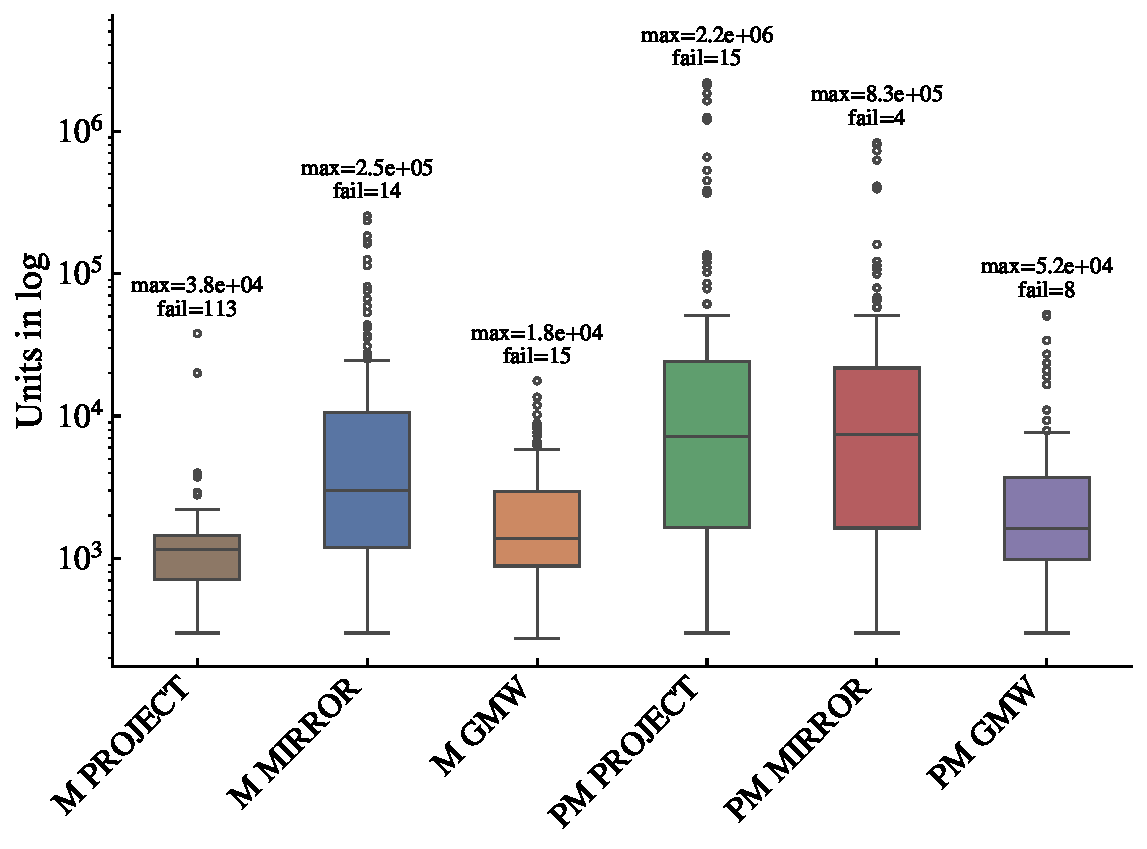
\includegraphics[width=0.8\textwidth]{images/experiment/Riccati-based_results/decomp_flop_worstcase_qp_results_riccati.pdf}
    \caption{Worst-case decomposition cost of the six Riccati-based methods (flops, log scale).
    Annotations report the maximum observed cost and the number of unsolved instances.}
    \label{fig:flop-profile-riccati}
\end{figure}

Taken together, two figures first reveal a robustness ordering,
\textsf{PM\_MIRROR} $>$ \textsf{PM\_GMW} $>$
\{\textsf{M\_MIRROR}, \textsf{M\_GMW}, \textsf{PM\_PROJECT}\} $>$ \textsf{M\_PROJECT}, 
where \textsf{PM\_PROJECT} only matches the plain \textsf{M} methods.
If reliability is the priority, \textsf{PM\_MIRROR} is the safest choice, as it leaves the fewest instances unsolved. 
If a balance between reliability and computational cost is preferred, \textsf{PM\_GMW} is the more attractive option, 
which maintains the robustness ($8$ unsolved instances) at a much lower worst-case cost.
We will therefore focus on \textsf{PM\_MIRROR} and \textsf{PM\_GMW} in the following comparisons with other regularization families.

\subsection{Comparison with full Hessian regularizations}
Having identified \textsf{PM\_MIRROR} and \textsf{PM\_GMW} as the strongest Riccati-based methods, 
we now compare them against the full Hessian regularizations.

The iteration profile in Figure~\ref{fig:iter-profile-fullhessian} 
shows the two Riccati-based methods sitting well above every full-Hessian variant across the whole iteration budget. 
\textsf{PM\_MIRROR} and \textsf{PM\_GMW} leave only $4$ and $8$ instances unsolved, 
whereas each \textsf{H} method leaves a substantial number of instances unsolved even at the largest budget. 
This suggests that regularizing the full Hessian does not recover 
the reliability or efficiency obtained by regularizing within the Riccati recursion.

\begin{figure}[H]
    \centering
    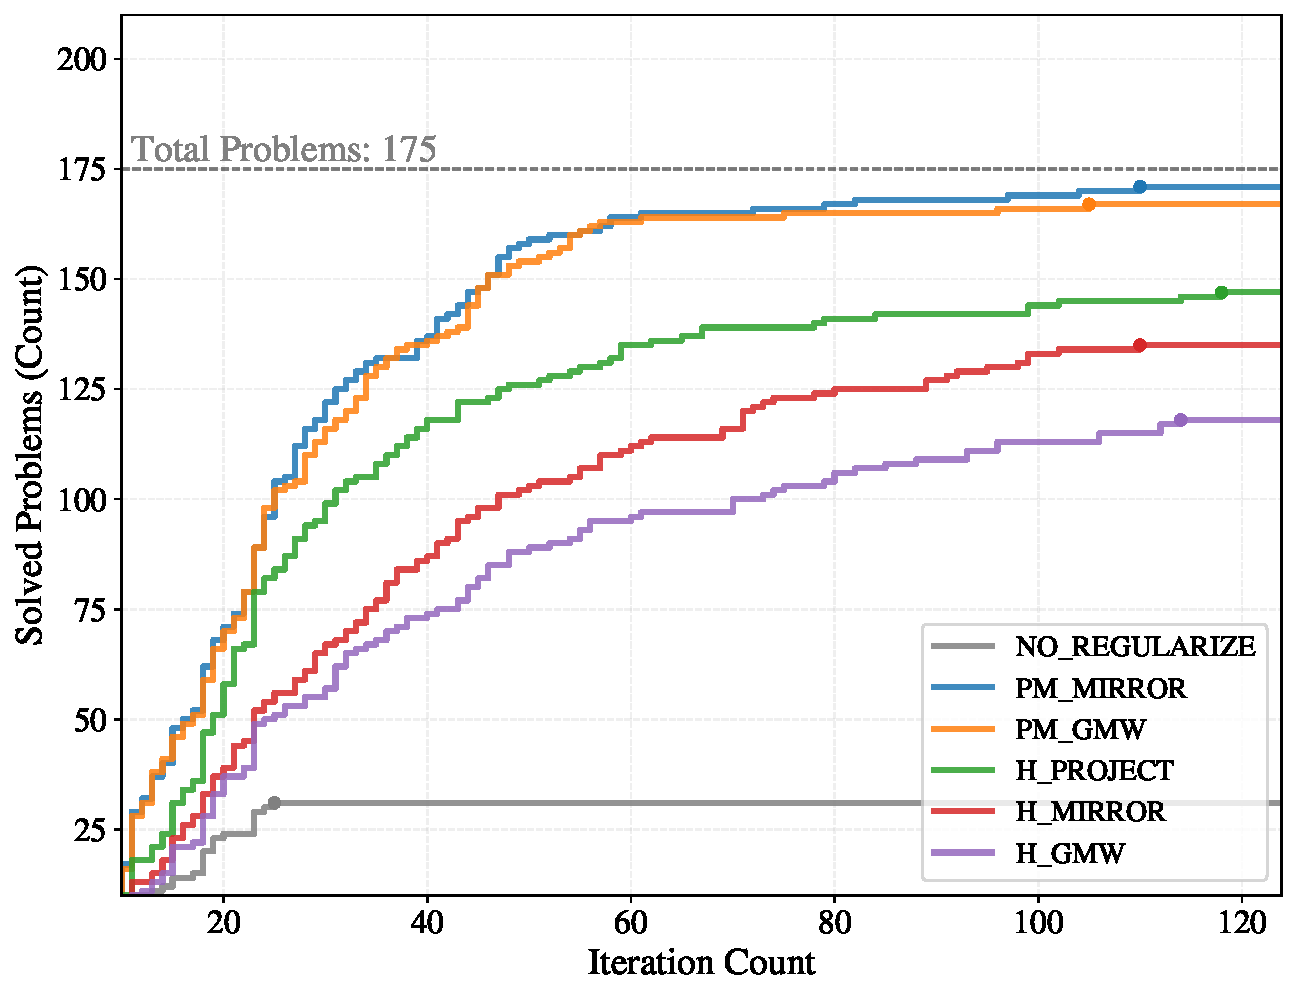
\includegraphics[width=0.8\textwidth]{images/experiment/Full_Hessian_results/iteration_qp_results_riccati.pdf}
    \caption{Iteration profile of the two strongest Riccati-based methods
    (\textsf{PM\_MIRROR}, \textsf{PM\_GMW}) against the full Hessian regularizations
    (\textsf{H\_PROJECT}, \textsf{H\_MIRROR}, \textsf{H\_GMW}).}
    \label{fig:iter-profile-fullhessian}
\end{figure}

In Figure~\ref{fig:flop-profile-fullhessian}, 
the gap between Riccati-based methods and Full Hesian methods is even more pronounced, 
and it runs in the Riccati-based methods' favour on \emph{both} axes. 
On the robustness, \textsf{PM\_MIRROR} fails on only $4$ instances and \textsf{PM\_GMW} on $8$, 
while the full-Hessian methods fail on $28$ (\textsf{H\_PROJECT}), $40$ (\textsf{H\_MIRROR}), and $57$ (\textsf{H\_GMW}) instances.
On the cost, the full-Hessian variants are also more expensive:
the worst-case costs of \textsf{H\_PROJECT} and \textsf{H\_MIRROR} lie far above those of both Riccati-based methods,
and even the cheapest full-Hessian option, \textsf{H\_GMW}, has a median cost well above that of \textsf{PM\_GMW},
yet it is also the least robust of the methods compared here. 
The full Hessian methods thus are considered neither speed nor reliability relative to the Riccati-based approach.

\begin{figure}[H]
    \centering
    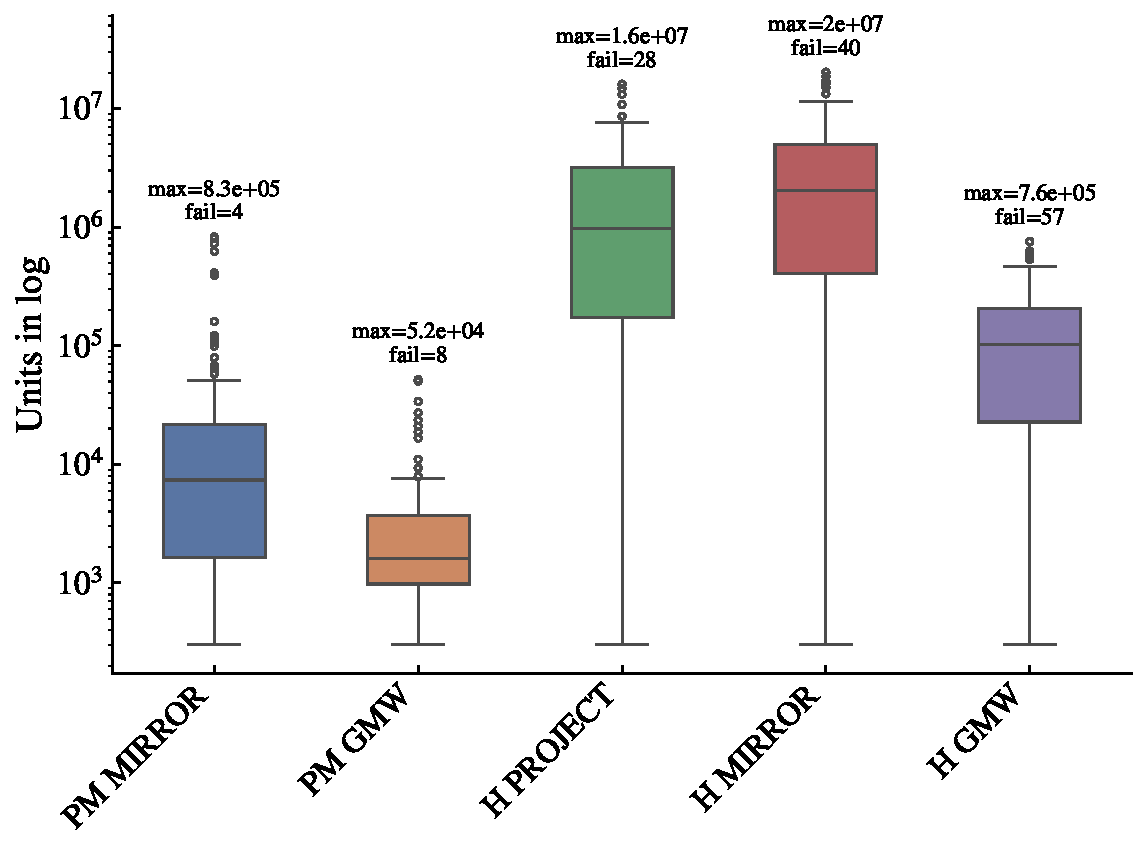
\includegraphics[width=0.8\textwidth]{images/experiment/Full_Hessian_results/decomp_flop_worstcase_qp_results_riccati.pdf}
    \caption{Worst-case decomposition cost of the two strongest Riccati-based methods
    against the full Hessian regularizations (flops, log scale).
    Annotations as in Figure~\ref{fig:flop-profile-riccati}.}
    \label{fig:flop-profile-fullhessian}
\end{figure}

The Riccati-based methods are simultaneously more robust and cheaper than every full-Hessian counterpart in Figure~\ref{fig:flop-profile-fullhessian}.
This supports the central premise of the approach, 
namely that regularizing the reduced Hessian by exploiting the stagewise structure of the problem is preferable to regularizing the full Hessian. 

\subsection{Comparison with inertia correction}
Finally, we compare the recommended Riccati-based methods against inertia
correction (\textsf{INERTIA\_LM}), which is widely used in practice and serves as a reference point for the comparison.

The iteration profiles in Figure~\ref{fig:iter-profile-inertia} end close for the three regularized methods, 
with \textsf{PM\_MIRROR} and \textsf{PM\_GMW} solving the most instances ($171$ and $167$) and \textsf{INERTIA\_LM} close behind ($164$). 
However, beyond about $25$ iterations the \textsf{PM\_MIRROR} and \textsf{PM\_GMW} sit clearly above \textsf{INERTIA\_LM}, 
indicating less iteration is needed to solve the same number of instances.

\begin{figure}[H]
    \centering
    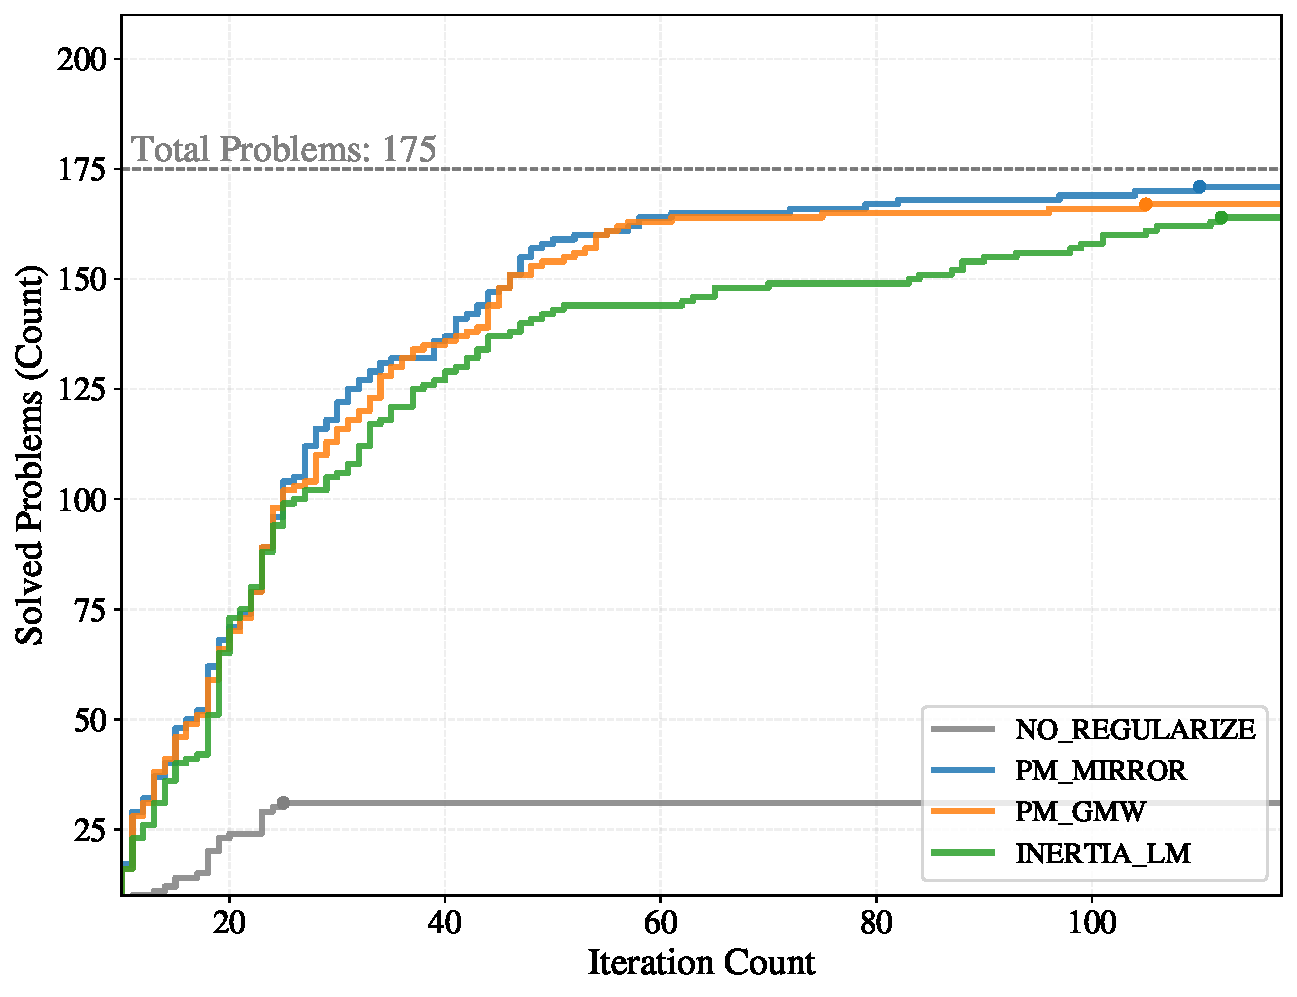
\includegraphics[width=0.8\textwidth]{images/experiment/Inertia_correction_results/iteration_qp_results_riccati.pdf}
    \caption{Iteration profile of \textsf{PM\_MIRROR} and \textsf{PM\_GMW}
    against inertia correction (\textsf{INERTIA\_LM}).}
    \label{fig:iter-profile-inertia}
\end{figure}

\begin{figure}[H]
    \centering
    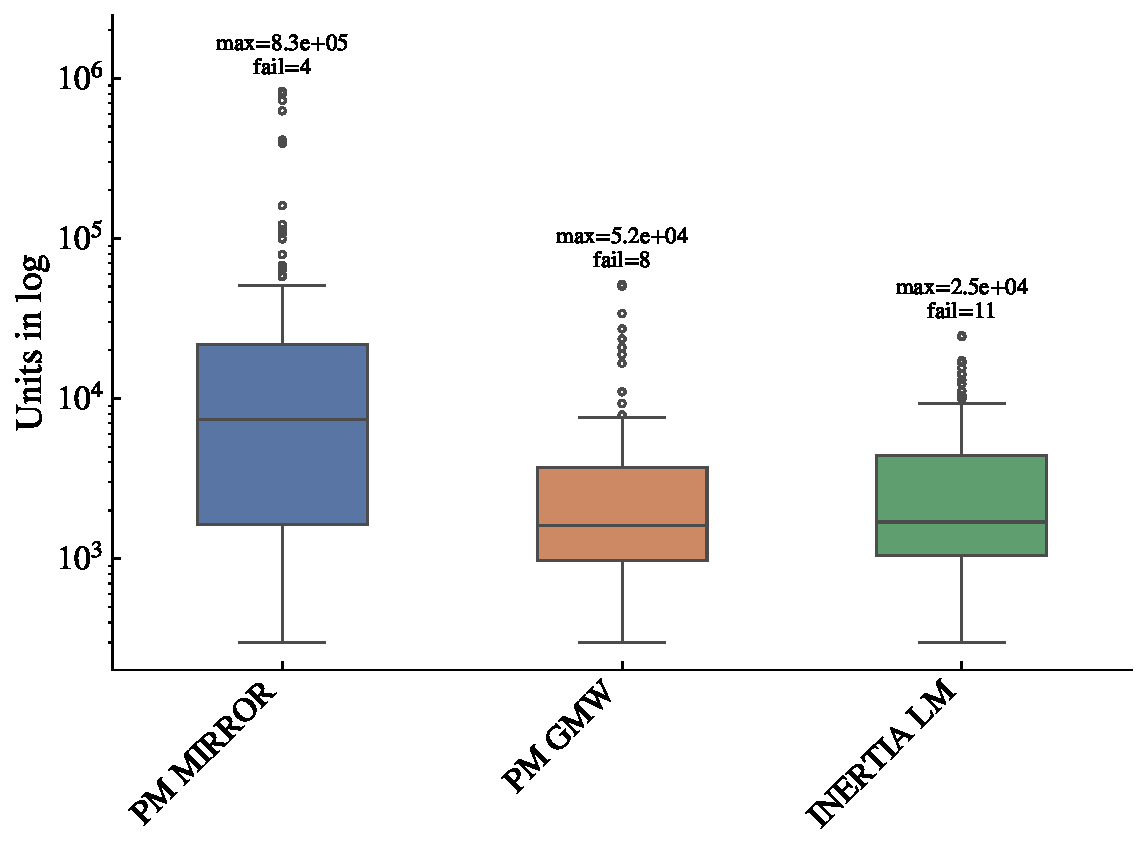
\includegraphics[width=0.8\textwidth]{images/experiment/Inertia_correction_results/decomp_flop_worstcase_qp_results_riccati.pdf}
    \caption{Worst-case decomposition cost of \textsf{PM\_MIRROR} and \textsf{PM\_GMW}
    against inertia correction (flops, log scale).
    Annotations as in Figure~\ref{fig:flop-profile-riccati}.}
    \label{fig:flop-profile-inertia}
\end{figure}

The decomposition-cost distribution in Figure~\ref{fig:flop-profile-inertia} draws the distinction more finely. 
Inertia correction is the cheapest of the three in the worst case, with a maximum cost of $2.5\times10^{4}$ flops, 
below both \textsf{PM\_GMW} ($5.2\times10^{4}$) and \textsf{PM\_MIRROR} ($8.3\times10^{5}$).
In terms of median cost, however, \textsf{INERTIA\_LM} and \textsf{PM\_GMW} are essentially on par, with \textsf{PM\_GMW} marginally lower. 
Their robustness differs more clearly, however: \textsf{INERTIA\_LM} fails on $11$ instances, against $8$ for \textsf{PM\_GMW} and $4$ for \textsf{PM\_MIRROR}.

From this benchmark, 
inertia correction is therefore preferable only where a hard bound 
on the per-decomposition cost outweighs the number of solved instances.

\subsection{Ablation on the conditional Mehrotra}
All results so far use Mehrotra's probing.
To justify this choice, we rerun \textsf{PM\_MIRROR}, \textsf{PM\_GMW}, \textsf{INERTIA\_LM} and \textsf{H\_PROJECT},
the most robust full Hessian variant, together with the unregularized baseline,
using the conditional predictor--corrector instead (\texttt{pred\_corr}$=$\texttt{cond\_pred\_corr}$=1$),
with all other settings unchanged.

\begin{figure}[H]
    \centering
    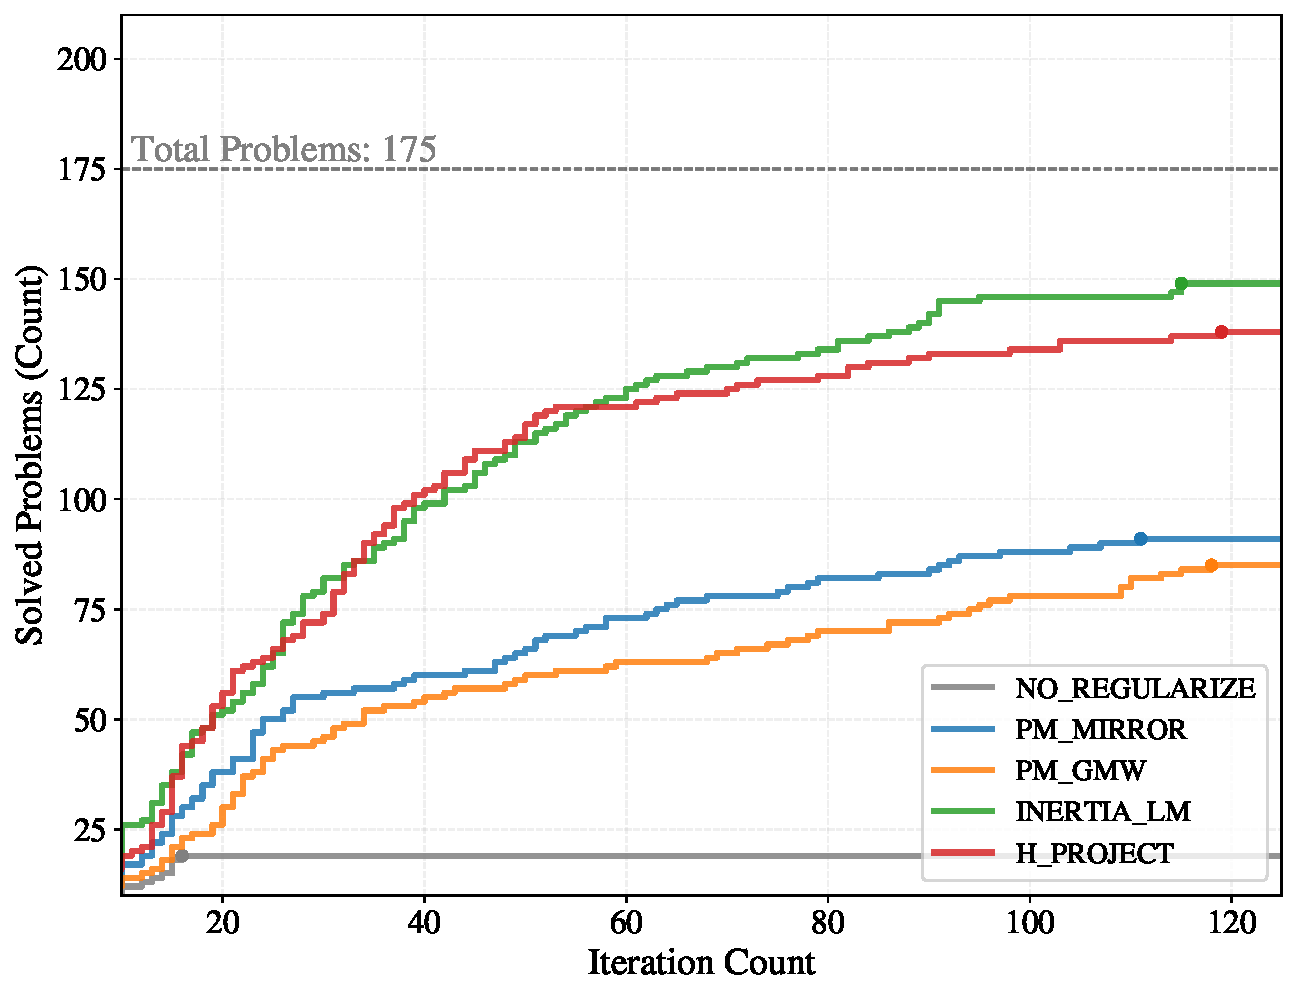
\includegraphics[width=0.8\textwidth]{images/experiment/ab_conditional_mehrotra/iteration_qp_results_riccati.pdf}
    \caption{Iteration profile with the conditional predictor--corrector
    of \textsf{PM\_MIRROR}, \textsf{PM\_GMW}, \textsf{INERTIA\_LM}, \textsf{H\_PROJECT} and the unregularized baseline.}
    \label{fig:iter-profile-corrector}
\end{figure}

Figure~\ref{fig:iter-profile-corrector} shows that every method solves fewer instances with the corrector, 
but the loss is far from uniform.
\textsf{PM\_MIRROR} and \textsf{PM\_GMW} drop from $171$ and $167$ to $91$ and $85$ solved instances,
whereas \textsf{INERTIA\_LM} and \textsf{H\_PROJECT} only drop from $164$ to $149$ and from $147$ to $138$.
The ranking of Section~\ref{sec:comparison} is thereby reversed,
and the two Riccati-based methods now trail both alternatives.
All additional failures exhaust the iteration budget,
and the worst-case decomposition cost in Figure~\ref{fig:flop-profile-corrector} rises for every method,
most visibly for \textsf{PM\_MIRROR}, whose maximum grows from $8.3\times10^{5}$ to $2.2\times10^{6}$ flops.

\begin{figure}[H]
    \centering
    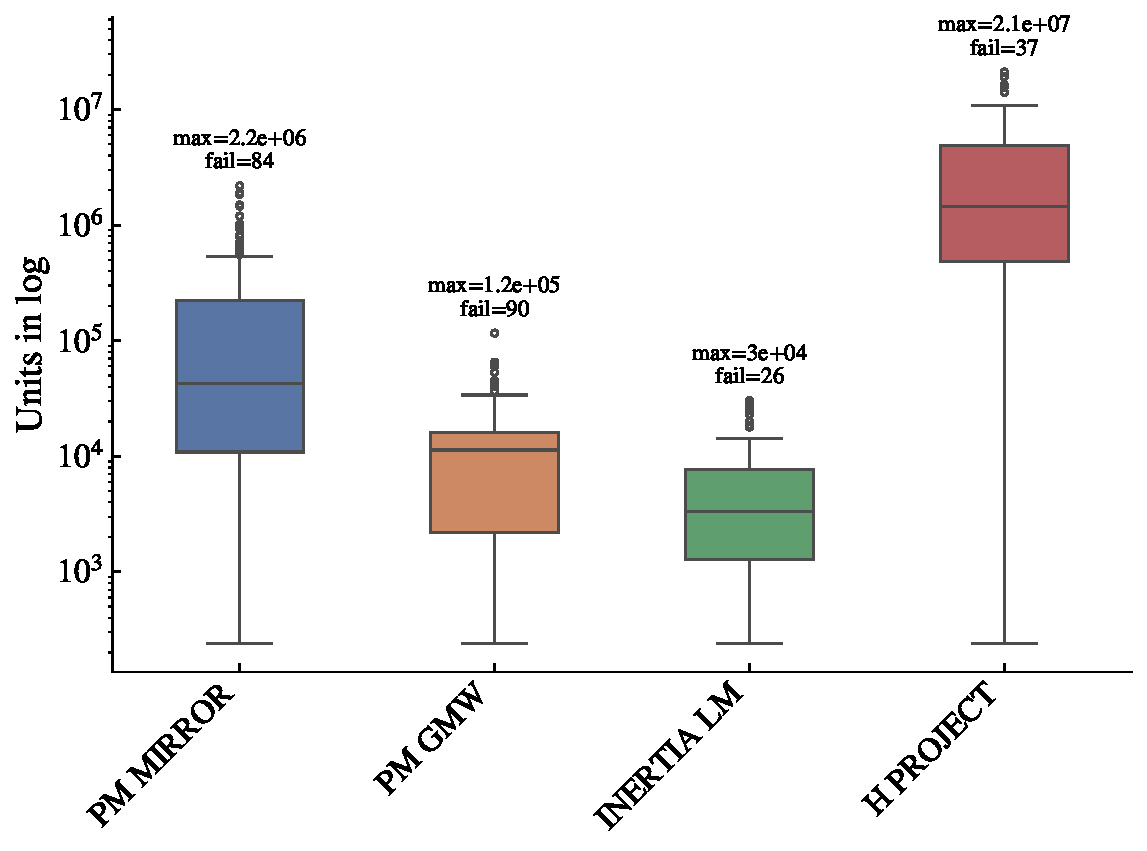
\includegraphics[width=0.8\textwidth]{images/experiment/ab_conditional_mehrotra/decomp_flop_worstcase_qp_results_riccati.pdf}
    \caption{Worst-case decomposition cost with the conditional predictor--corrector (flops, log scale).
    Annotations as in Figure~\ref{fig:flop-profile-riccati}.}
    \label{fig:flop-profile-corrector}
\end{figure}

This is consistent with the argument in Section~\ref{sec:update}
and is why probing is adopted as the default barrier update in all other experiments.
Section~\ref{subsec:ablation_analysis} discusses why \textsf{PM\_MIRROR} loses far more instances than \textsf{INERTIA\_LM}.

\subsection{Ablation on the line search}
The two-phase line search of Section~\ref{subsec:two_phase_search} was introduced to safeguard the FTB step on nonconvex QPs.
To isolate its contribution, we disable it, so that the FTB step is taken directly,
and rerun the same five methods as in the previous subsection with all other settings unchanged.

\begin{figure}[H]
    \centering
    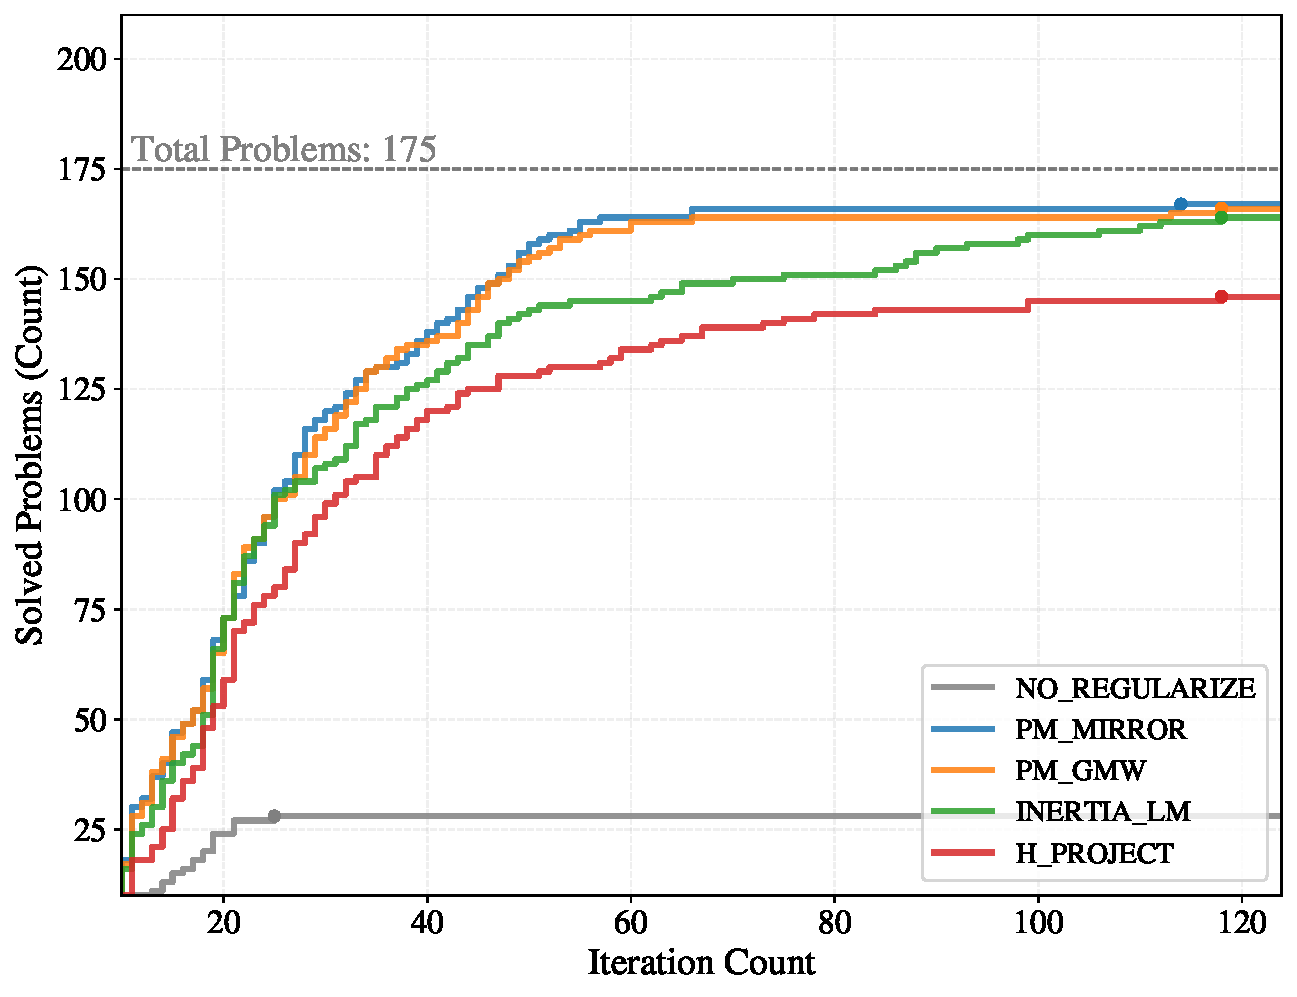
\includegraphics[width=0.8\textwidth]{images/experiment/ab_line_search_results/iteration_qp_results_riccati.pdf}
    \caption{Iteration profile without the line search
    of \textsf{PM\_MIRROR}, \textsf{PM\_GMW}, \textsf{INERTIA\_LM}, \textsf{H\_PROJECT} and the unregularized baseline.}
    \label{fig:iter-profile-nols}
\end{figure}

\begin{figure}[H]
    \centering
    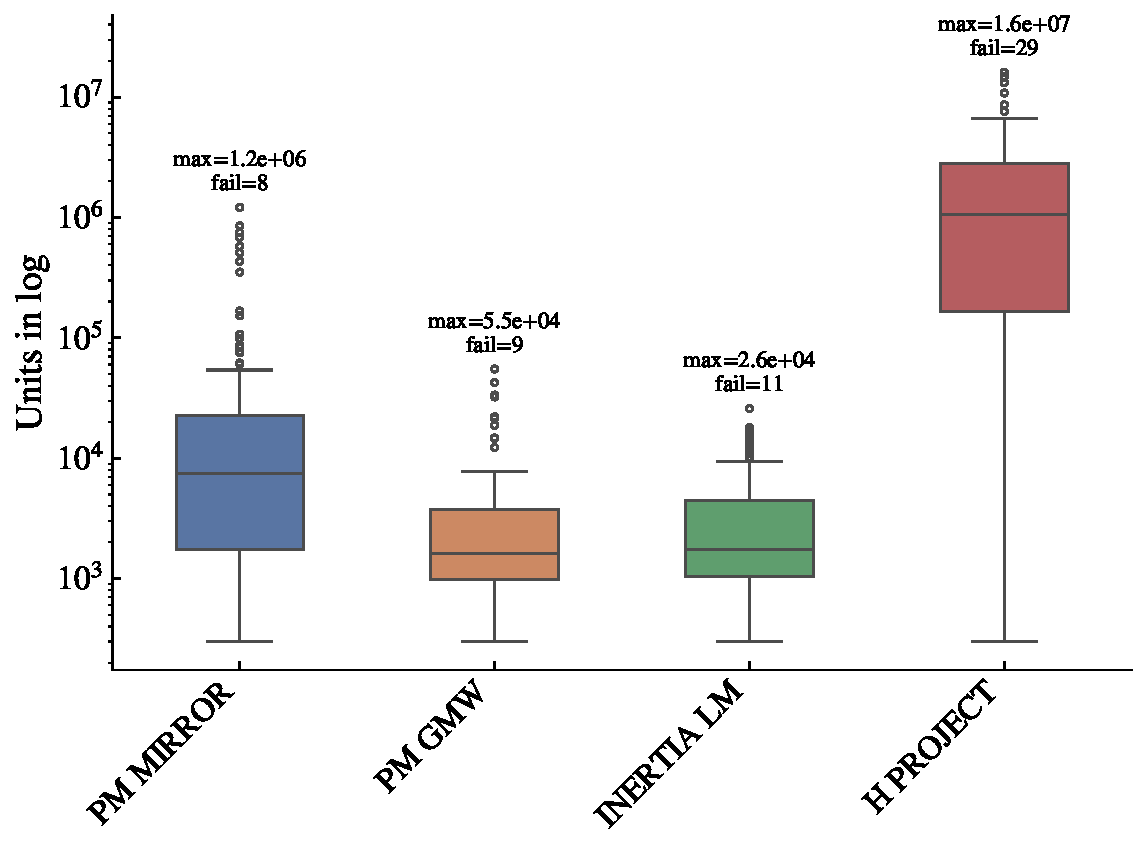
\includegraphics[width=0.8\textwidth]{images/experiment/ab_line_search_results/decomp_flop_worstcase_qp_results_riccati.pdf}
    \caption{Worst-case decomposition cost without the line search (flops, log scale).
    Annotations as in Figure~\ref{fig:flop-profile-riccati}.}
    \label{fig:flop-profile-nols}
\end{figure}

Figure~\ref{fig:iter-profile-nols} shows that the line search has a much smaller effect than the choice of barrier update.
Without it, \textsf{PM\_MIRROR} solves $167$ instead of $171$ instances,
\textsf{PM\_GMW} $166$ instead of $167$ and \textsf{H\_PROJECT} $146$ instead of $147$,
while \textsf{INERTIA\_LM} solves $164$ in both cases.
\textsf{PM\_MIRROR} benefits most, as the line search adds four solved instances and loses none,
whereas for the other methods the instances it gains and loses nearly cancel.
On the instances solved in both settings, most iteration counts are identical.
The worst-case decomposition cost in Figure~\ref{fig:flop-profile-nols} also stays close to that with the line search,
apart from the maximum of \textsf{PM\_MIRROR}, which rises from $8.3\times10^{5}$ to $1.2\times10^{6}$ flops.

The ranking of Section~\ref{sec:comparison} therefore does not rely on the line search.
The robustness of the Riccati-based methods stems from the regularization itself,
and Section~\ref{subsec:ablation_analysis} discusses why the line search mainly helps \textsf{PM\_MIRROR}.

\section{Discussion}
\label{sec:discussion}
The comparison in Section~\ref{sec:comparison} counted the unsolved instances of each method.
This section first resolves these failures along two directions.
Section~\ref{subsec:failure_status} splits them by the status with which the solve terminated,
which separates a numerical breakdown of the regularized recursion
from a mere exhaustion of the iteration budget.
Section~\ref{subsec:failure_category} splits them by the OCP each instance was collected from,
which identifies what distinguishes the hard instances from the easy ones and explains why some methods perform poorly.
Finally, Section~\ref{subsec:ablation_analysis} explains why the ablations of the barrier update and the line search
affect \textsf{PM\_MIRROR} and \textsf{INERTIA\_LM} so differently.

\subsection{Failure by status}
\label{subsec:failure_status}
A run that does not converge ends with one of three exit statuses,
shown per method in Figure~\ref{fig:failures-by-status}:
\begin{itemize}
    \item \emph{Unregularized}: the Cholesky factorization fails \emph{again} after the regularization has been applied, 
    usually caused by numerical indefiniteness.
    \item \emph{Max iterations reached}: the residuals did not fall below their tolerances within the budget $i_\mathrm{max}=120$.
    \item \emph{NaN encountered}: an infinite or undefined value appeared in the residuals, so that the iterate itself has overflowed.
\end{itemize}

In Figure~\ref{fig:failures-by-status}, 
the \textsf{M\_PROJECT} is the only Riccati-based method with numerical breakdowns with $113$ of its $175$ instances unsolved.
$110$ of its $113$ failures stem from numerical issue, 
while only $3$ exhaust the iteration budget.
This confirms the analysis in Section~\ref{sec:fail_minimal_perturbation}, 
where ill-conditioning propagates into numerical indefiniteness or overflow.
Adopting either remedy identified there resolves these breakdowns: 
abandoning the minimum-perturbation rule (\textsf{M\_MIRROR}, \textsf{M\_GMW}) 
or adding the cost-to-go correction (\textsf{PM\_PROJECT}) eliminates all NaN and unregularized failures,
leaving only iteration-limit terminations ($14$, $15$, and $15$ failures, respectively).
Combining both remedies, 
as in \textsf{PM\_MIRROR} and \textsf{PM\_GMW}, further reduces the remaining iteration-limit failures.
\textsf{INERTIA\_LM} likewise fails only by reaching the iteration limit.

\begin{figure}[H]
    \centering
    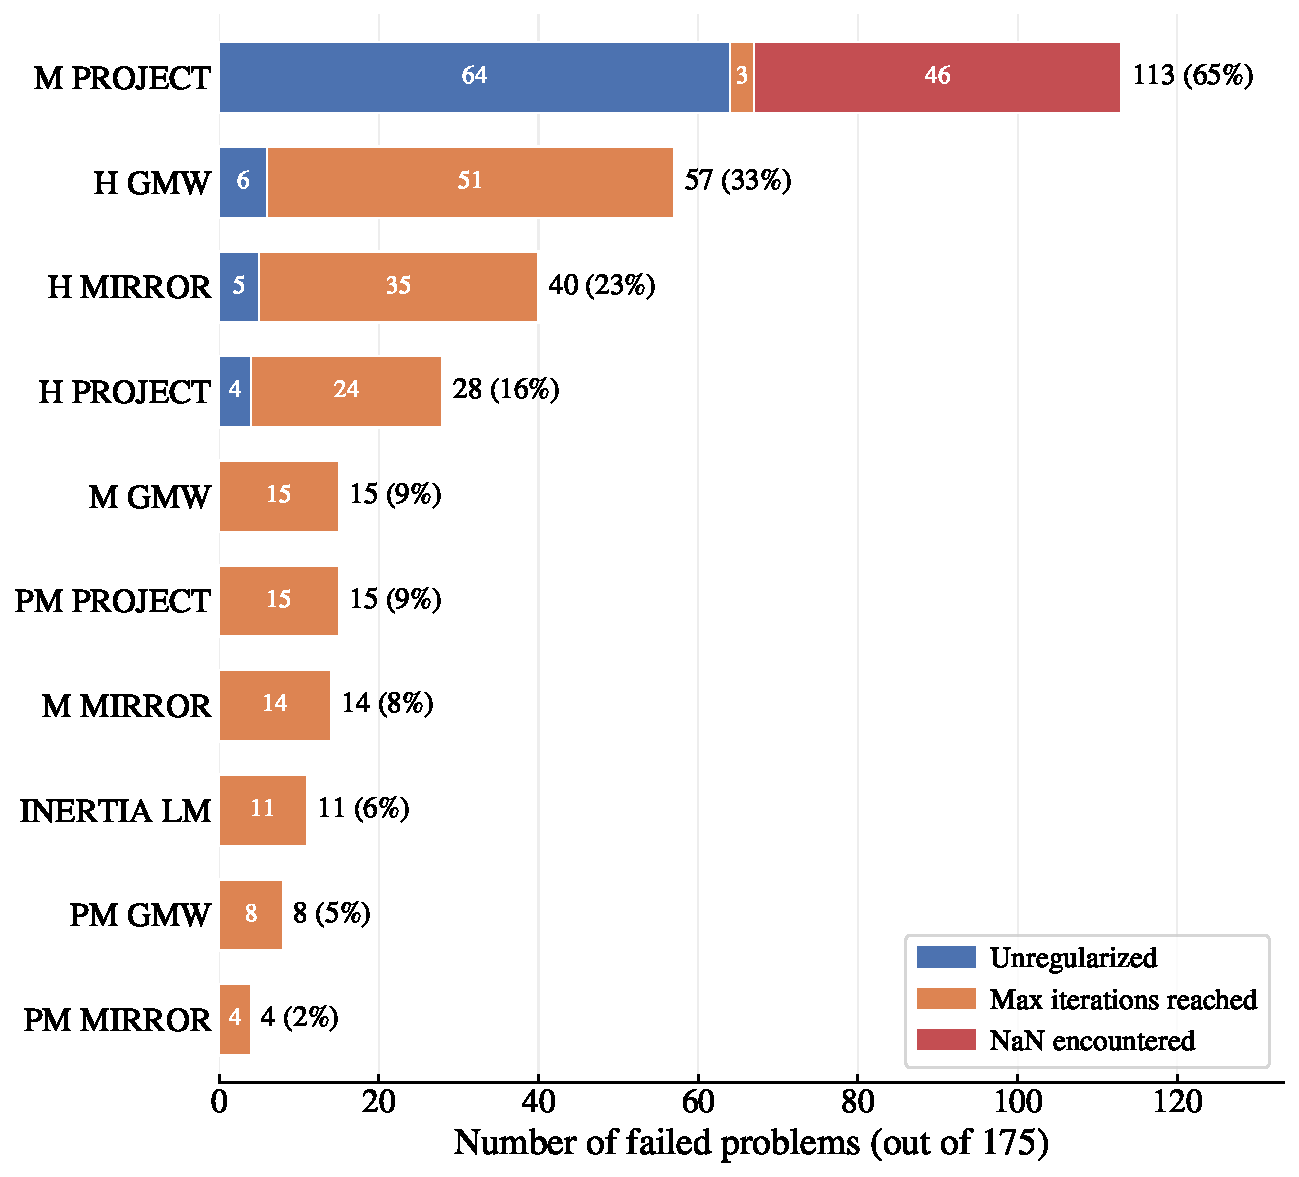
\includegraphics[width=0.85\textwidth]{images/experiment/discussion/qp_failures_by_status.pdf}
    \caption{Failures of each method by exit status over the $175$-instance test set.
    The bars are stacked by status and annotated with the total number of unsolved instances
    and the corresponding share of the test set.}
    \label{fig:failures-by-status}
\end{figure}

The full Hessian methods break down on $4$, $5$ and $6$ instances,
but most of their failures reach the iteration limit ($24$, $35$ and $51$).
Their breakdowns come from the cost-to-go matrix $P_k$, which no \textsf{H} strategy modifies.
Near convergence, the barrier term $\Lambda_k T_k^{-1}$ grows as the slacks of active constraints approach zero,
and the Riccati recursion carries this growth into $P_k$.
Once $\kappa_2(P_k)\,\epsilon_{\mathrm{mach}} \ge 1$, where $\epsilon_{\mathrm{mach}}$ denotes the machine precision,
rounding errors exceed the smallest eigenvalue of $P_k$, and the computed $P_k$ can become indefinite.
The Riccati-based methods meet the same $P_k$ but do not require $P_k \succ 0$,
since they enforce $\tilde{M}_k \succ 0$ before each Cholesky factorization.

Accordingly, for the six methods that never suffer factorization breakdowns,
namely the Riccati-based methods other than \textsf{M\_PROJECT} together with \textsf{INERTIA\_LM},
all failures reduce strictly to exhausted iteration limits,
which plausibly reflect an inadequate regularization scale or an ineffective search direction.

\subsection{Failure by category}
\label{subsec:failure_category}
Figure~\ref{fig:failures-by-category} resolves the same failures by the OCP each instance was collected from.
The cell entries are the numbers of unsolved instances and the shading is the failure rate within the column,
so that categories of different size remain comparable,
and the eight columns are ordered by size and sum to the $175$ instances of the test set.

\begin{figure}[H]
    \centering
    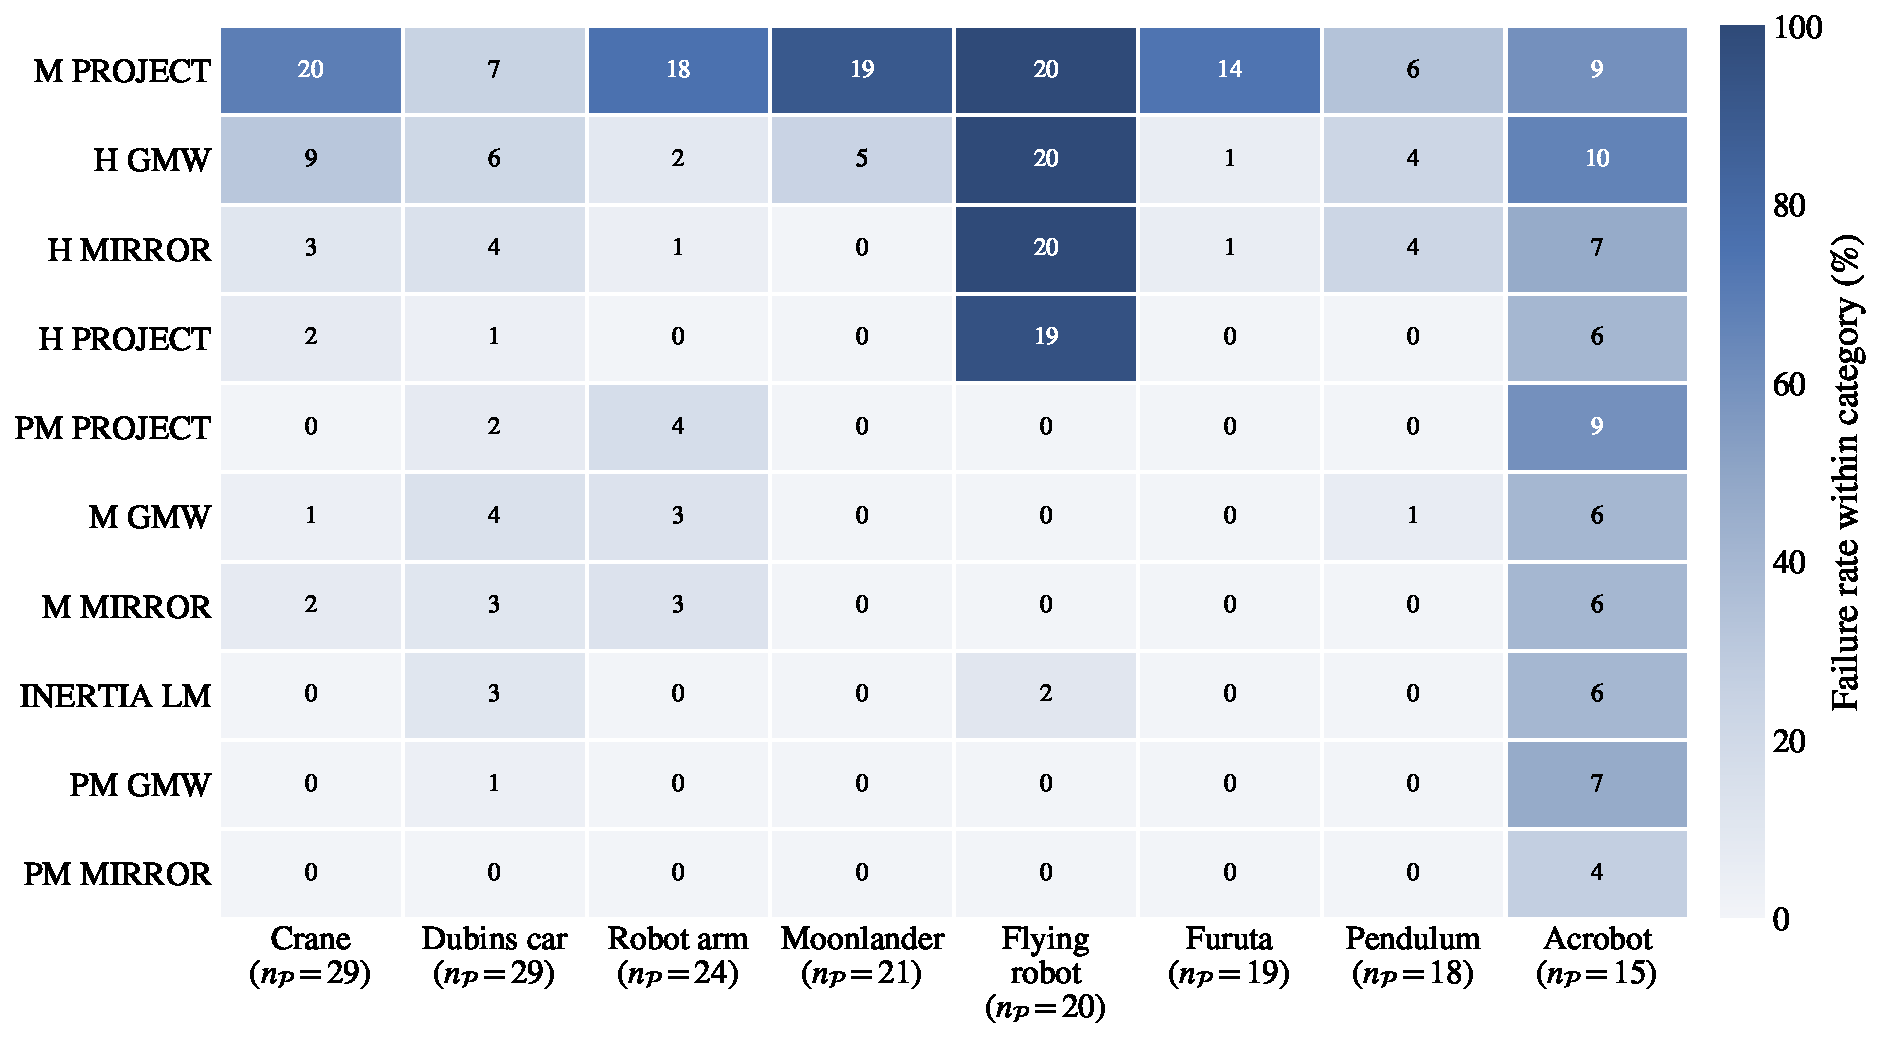
\includegraphics[width=1.0\textwidth]{images/experiment/discussion/qp_failures_by_category.pdf}
    \caption{Failures of each method by OCP category.
    The cell entries give the number of unsolved instances and the shading gives the failure rate within the column,
    where $n_\mathcal{P}$ is the number of instances collected from that OCP.
    The rows are ordered by total failure count and the columns by size.}
    \label{fig:failures-by-category}
\end{figure}

Comparing with Figure~\ref{fig:indefinite_qp_scatter} suggests that an instance becomes hard
when its indefiniteness is both deep and wide.
Two \textsl{Crane} instances with very deep negative curvature are indefinite in only $5\%$ and $7\%$ of their stages,
and every method except \textsf{M\_PROJECT} and \textsf{H\_GMW} solves both:
the isolated indefinite stage is corrected once and the recursion recovers.
The four unsolved \textsl{Acrobot} instances instead have $|\lambda_{\min}| > 250$ in $33\%$ to $53\%$ of their stages,
so large corrections are needed at many stages, and no method converges within the iteration budget.
No other OCP in Figure~\ref{fig:indefinite_qp_scatter} combines such depth with such a rate.

For the full Hessian methods, \textsl{Flying robot} is the hardest OCP:
\textsf{H\_PROJECT}, \textsf{H\_MIRROR} and \textsf{H\_GMW} fail on $19$, $20$ and $20$ of its $20$ instances,
while every Riccati-based method except \textsf{M\_PROJECT} solves all of them.
In \textsl{Flying robot}, the indefiniteness lies only in the cost-to-go matrix and affects about $2\%$ of the stages,
while $R_k \succ 0$ throughout (Figure~\ref{fig:indefinite_source_signature}).
The full Hessian methods cannot act on $P_k$, so they perturb $\tilde{Q}_k$ over the whole horizon,
including the stages that need no correction, and exhaust the iteration budget.
This supports the premise of Section~\ref{sec:riccati_primal_reg}
that indefiniteness should be treated where it arises in the recursion.

\textsf{INERTIA\_LM} adds $\delta_w I$ to both $\tilde{Q}_k$ and $\tilde{R}_k$,
which in the Riccati recursion shifts both $P_k$ and $\tilde{M}_k$.
It therefore solves $18$ of the $20$ \textsl{Flying robot} instances,
and its total failure count is much closer to the \textsf{PM} methods than to the full Hessian ones.
Unlike the Riccati-based methods, however, its shift is not localized:
$\delta_w$ must be large enough for the most negative eigenvalue over all stages and is applied at every stage.

The figure also refines the \textsf{M} versus \textsf{PM} comparison of Section~\ref{sec:comparison}.
\textsf{M\_MIRROR} and \textsf{M\_GMW} already solve every \textsl{Flying robot} instance.
Apart from \textsl{Acrobot}, their failures lie mainly on \textsl{Dubins car}, \textsl{Crane} and \textsl{Robot arm},
two of which are dominated by the \emph{both} case, where $R_k$ and $P_{k+1}$ are indefinite at the same stage.
\textsf{PM\_MIRROR} solves all instances of these three OCPs and \textsf{PM\_GMW} fails on only one \textsl{Dubins car} instance,
consistent with the propagation through $P_k$ predicted in Section~\ref{sec:fail_minimal_perturbation}.

In summary, the instances that no method solves combine deep negative curvature with many indefinite stages,
which in this benchmark occurs only in \textsl{Acrobot}.
The full Hessian methods underperform because enforcing $\tilde{H}_k \succ 0$ alters the state curvature
even when only a few stages are indefinite, as in \textsl{Flying robot}.
Regularizing within the Riccati recursion avoids this by modifying only the indefinite matrices at the stages where they arise,
although the \textsl{Acrobot} instances remain unsolved by all methods.


\subsection{Analysis on ablation}
\label{subsec:ablation_analysis}
Based on the two ablations, this subsection explains the behavior of \textsf{PM\_MIRROR} and \textsf{INERTIA\_LM}
by addressing two questions:
\begin{enumerate}
    \item Why does the ranking of Section~\ref{sec:comparison} reverse under the conditional Mehrotra corrector?
    \item Why does the line search mainly help \textsf{PM\_MIRROR} but not \textsf{INERTIA\_LM}?
\end{enumerate}

Recall \eqref{eq:schur_comp_KKT_reduced}. With simplified notation, the
regularized system reads
\begin{equation}
    (\tilde{M}_i + E_i) \Delta y_z = -r_i,
    \label{eq:schur_comp_KKT_reduced_simple_reg}
\end{equation}
and the step is bounded by
\begin{equation}
    \|\Delta y_z\| \le \frac{\|r_i\|}{\lambda_{\min}(\tilde{M}_i+E_i)}.
    \label{eq:step_bound}
\end{equation}
The bound holds for both methods, which differ in how small $\lambda_{\min}(\tilde{M}_i+E_i)$ can become.

\textsf{INERTIA\_LM} increases a uniform shift $\delta$ until the factorization succeeds. 
If $\delta_{\min}$ is the smallest shift for which it succeeds, then $\lambda_{\min}(\tilde{M}_i+E_i) \ge \delta-\delta_{\min}$. 
Since the shift is increased by the factor $\kappa_w^+$, 
the accepted $\delta$ usually lies well above $\delta_{\min}$, and $\lambda_{\min}$ stays of the order of $\delta$.

\textsf{PM\_MIRROR} modifies only the negative eigenvalues of $M_k$ and $P_k$, stage by stage. 
A small positive pivot passes the factorization unmodified and can produce large feedback gains, 
so nothing prevents $\lambda_{\min}(\tilde{M}_i+E_i)$ from approaching zero.
On regularized iterations, 
\textsf{PM\_MIRROR} reaches a much smaller $\lambda_{\min}(\tilde{M}_i+E_i)$ than \textsf{INERTIA\_LM} at similar $\|r_i\|$, 
and its affine steps are correspondingly longer, thus a full affine step could be impossible to be performed.

\paragraph{On the Barrier Update Strategies.}
Mehrotra's corrector adds the second-order term
$\Delta T_{\mathrm{aff}}\Delta\Lambda_{\mathrm{aff}}\mathbf{1}$ to the right-hand side,
which grows quadratically with the affine step.
As shown in Table~\ref{tab:step_metrics}, the median affine step of \textsf{PM\_MIRROR} is far longer than that of \textsf{INERTIA\_LM}.

In \textsf{PM\_MIRROR},
the second-order term then dominates the right-hand side and results a long corrector step,
the fraction-to-boundary rule, thus, leaves only a very short step size.
Since, the affine step is itself cut short, $\mu_{\mathrm{aff}}$ stays close to $\mu$,
and the very short corrected step leaves $\mu_{\mathrm{cor}}$ close to $\mu$ as well, below $2\mu_{\mathrm{aff}}$.
The safeguard of Section~\ref{sec:update} rarely detects this, 
so the bad corrector step is taken,
which is dominated by a correction for the second-order error of an affine step that cannot be taken, 
so it neither reduces the residuals nor moves the iterate along the directions needed to leave the indefinite region.

\textsf{INERTIA\_LM} lifts every direction by the uniform shift $\delta I$,
which keeps $\lambda_{\min}$ away from zero and the affine step moderate.
The second-order term therefore stays comparable in size to the rest of the right-hand side,
so the corrected direction remains moderate as well,
and the fraction-to-boundary rule leaves a step size comparable to that of a centering step.
Since $\mu_{\mathrm{aff}}$ then lies clearly below $\mu$, the safeguard is effective and rejects $39.1\%$ of the corrector steps.
The conditional corrector step thus makes progress as intended,
and \textsf{INERTIA\_LM} loses far fewer instances to the corrector than \textsf{PM\_MIRROR}.

With probing, the affine step only determines the centering parameter,
so the second-order term no longer enters the search direction, and the ranking reverses.
The shift $\delta I$ in \textsf{INERTIA\_LM} raises the curvature of directions
that are already positive, which shortens the step along weakly curved directions.
\textsf{INERTIA\_LM} therefore moves less per regularized iteration and needs more of them, 
as one can see in Table~\ref{tab:step_metrics}.
\textsf{PM\_MIRROR}, in contrast, keeps its steps along weakly curved directions long.
Without the second-order term, these long steps no longer distort the search direction,
so \textsf{PM\_MIRROR} moves further per regularized iteration,
leaves the region where the reduced Hessian is indefinite sooner,
and reaches the regime where unregularized Newton steps converge quickly.

\begin{table}[H]
\centering
\caption{Step metrics of \textsf{PM\_MIRROR} and \textsf{INERTIA\_LM}.}
\label{tab:step_metrics}
\vspace{0.5em}
\begin{tabular}{lcc}
\toprule
 & \textsf{PM\_MIRROR} & \textsf{INERTIA\_LM} \\
\midrule
\multicolumn{3}{l}{\emph{Corrector, on $175$ instances}} \\
\quad Median affine step $\|\Delta y_z\|$             & $65.4$ & $4.4$ \\
\quad Percentage of rejected corrector steps          & 3.7\,\% & 39.1\,\% \\
\addlinespace
\multicolumn{3}{l}{\emph{Probing, on $164$ instances solved by both}} \\
\quad Iterations                                      & $4218$ & $5132$ \\
\quad Regularized iterations                          & $1566$ & $2289$ \\
\quad Median displacement $\alpha_{\mathrm{prim}}\|\Delta y_z\|$ & $1.44$ & $0.47$ \\
\bottomrule
\end{tabular}
\end{table}

\paragraph{On the Line Search.}
The two-phase line search distinguishes three situations:
\begin{enumerate}
    \item high infeasibility or an ascent direction, handled by an h-phase step;
    \item moderate or low infeasibility, handled by an f-phase step;
    \item feasibility, handled by an f-phase step.
\end{enumerate}
Since the constraints are affine, every step scales the violation as $\theta^{+} = (1-\alpha_{\mathrm{prim}})\,\theta$,
so the line search never has to enforce feasibility.
Backtracking in the f-phase is triggered only by the barrier objective,
when the fraction-to-boundary rule drives a slack close to its bound 
and the barrier increase exceeds the predicted decrease $\alpha_{\mathrm{prim}}|\rho|$ of a short step.

In \textsf{PM\_MIRROR}, the short step size corresponding to the long regularized directions barely reduce $\theta$, 
so \textsf{PM\_MIRROR} remains in situation 2 throughout its regularized iterations.
A trial step there predicts little decrease, so the Armijo condition rejects it, 
and backtracking keeps the blocking slack off its bound.

\textsf{INERTIA\_LM} shifts the curvature of all directions uniformly,
which keeps its directions short, so the fraction-to-boundary rule rarely cuts them.
The predicted decrease of these long steps outweighs the barrier increase, so the f-phase rarely backtracks,
and the instances the line search gains and loses for \textsf{INERTIA\_LM} cancel.

\end{document}
